\documentclass[]{article}
% \includeonly{chapters/3-malicious.tex}


\usepackage[utf8]{inputenc}
% formatting imports
\usepackage{graphicx}
\usepackage[margin=1cm]{caption}
\usepackage[a4paper, total={6in, 8in}]{geometry}
\usepackage[section]{placeins}
\usepackage{array}

\usepackage{setspace}
\setlength{\parskip}{1em}

% math imports
\usepackage{siunitx}
\usepackage{amsmath}
\usepackage{amsthm}
\usepackage{amssymb}
\usepackage{mathtools}
\usepackage{bbold}



\usepackage{hyperref}
\hypersetup{
    colorlinks,
    citecolor=black,
    filecolor=black,
    linkcolor=black,
    urlcolor=black
}

\usepackage{listings}
\lstset{basicstyle=\footnotesize\ttfamily,breaklines=true}
\lstset{framextopmargin=50pt,frame=bottomline}

\usepackage{tikz}
\usepackage{longtable}
\usetikzlibrary{arrows}

\usepackage[sorting=none]{biblatex}
\addbibresource{refs.bib}

% \usepackage[textsize=tiny]{todonotes}
% \newcommand{\todoref}[2][]{\todo[color=cyan!40, #1]{\textbf{ref:}\\#2}}
% \newcommand{\todoidkcite}[2][]{\todo[color=cyan!10, #1]{\textbf{ref:}\\#2}}
% \newcommand{\todofig}[2][]{\todo[color=red!40, #1]{\textbf{fig:}\\#2}}
% \newcommand{\todoidea}[2][]{\todo[color=green!40, #1]{\textbf{idea:}\\#2}}
% \newcommand{\todoexplain}[2][]{\todo[color=purple!40, #1]{\textbf{details:}\\#2}}
% \newcommand{\todooptional}[2][]{optional \todo[color=grey!10, #1]{#2}}

\newcommand{\todoref}[2][]{}
\newcommand{\todoidkcite}[2][]{}
\newcommand{\todofig}[2][]{}
\newcommand{\todoidea}[2][]{}
\newcommand{\todoexplain}[2][]{}
\newcommand{\todooptional}[2][]{}
\newcommand{\todo}[2][]{}
\newcommand{\listoftodos}[2][]{}

\usepackage{subfigure}
% green!40]

\usepackage[fontsize=12pt]{fontsize}

\newcommand{\del}[2]{\frac{\partial #1}{\partial #2}}
\newcommand{\delsquare}[2]{\frac{\partial^2 #1}{\partial #2 ^2}}

\newcommand{\full}[2]{\frac{d #1}{d #2}}
\newcommand{\fullsquare}[2]{\frac{d^2 #1}{d #2 ^2}}

\newcommand{\ccf}[1]{`\cf{#1}'}
\newcommand{\cf}[1]{\textnormal{\textsf{#1}}}

\newcommand{\amps}[0]{\ampere}
\newcommand{\muamps}[0]{\micro\ampere}

\title{IGNORE THIS PAGE IN CURRENT VERSION}

\DeclareUnicodeCharacter{2212}{-}
\DeclarePairedDelimiter\ceil{\lceil}{\rceil}
\DeclarePairedDelimiter\floor{\lfloor}{\rfloor}
\begin{document}

% \listoftodos

\doublespacing

\maketitle

\begin{center}
    Massachusetts Institute of Technology \\
    Department of Electrical Engineering and Computer Science
\end{center}

\begin{center}
    Proposal for Thesis Research in Partial Fulfillment\\ of the Requirements for the Degree of\\
Masters of Engineering
\end{center}

\vfill

\begin{tabular}{rl}
\textbf{Title:} & \textbf{Defect Identification in Superconducting 2-Terminal Devices} \\
\\
\textbf{Submitted by:} & T. Dandachi \\
              & 69 Chestnut St. \\
              & Cambridge, MA 02139
\end{tabular}

\vspace{15mm}
\begin{tabular}{@{}p{1.5in}p{4in}@{}}
\textbf{Signature of author:} & \hrulefill \\
\end{tabular}

\vfill

\textbf{Expected Date of Completion:} May 2022

\vfill

\textbf{Laboratory:} Quantum Nanostructures and Nanofabrication under the Research Laboratory for Electronics

\vfill

\textbf{Abstract:}

Simulating the operation of a superconducting device

\vfill

\textbf{Supervision Agreement:}

The program outlined in this proposal is adequate for a Master's thesis. The supplies and facilities required are available, and I am willing to supervise the research and evaluate the thesis report.

\vspace{15 mm}
\begin{tabular}{@{}p{1.5in}p{4in}@{}}
  & \hrulefill \\
& K. K. Berggren, Prof. of Elec. Eng.
\end{tabular}

\newpage

\tableofcontents

\listoffigures

\newpage

% figures are here: https://www.icloud.com/keynote/094kHrSTQlvohxqCHGUmZJXcg#thesis

\section{Introduction}

The non-linear behavior of superconducting nanowires is a crucial aspect of many of their applications, including superconducting nanowire single-photon detectors (SNSPDs) and neuromorphic computing \cite{snspd_original_paper, spiking_nn}. However, this non-linearity also makes it challenging to simulate nanowires, particularly when considering their microwave properties. One common method of simulating these nanowire electronics relies on existing circuit simulation environments \cite{karl_spice}. These environments were optimized for classical electronics and lack optimizations that account for the microwave and superconducting characteristics of the models.

While plenty of good superconducting simulators exist for the frequency domain
modeling of devices, they tend to neglect effects that nanowire-based device 
designer care about \cite{josephsoncircsjl, wrspice}. These effects include simulating pulses, thermal modeling
of hotspot generation, and thermal coupling in stacks.
Simulating the dominant effects in our superconducting electronics in the time domain
is a crucial step for device design.

As we scale device sizes and introduce dependence on thermal effects and electrostatic coupling, the complexity of the models makes it increasingly difficult to accurately and efficiently simulate the device's time behavior properly.
While the need for more accurate nanowire simulations and the complexity of our models continue to grow, the tools used to simulate these devices must also evolve to meet these challenges. We aim to address that
by introducing wrappers around existing SPICE software, a method for quickly
assessing simulation stability and present the building blocks for a new
nanowire electronics simulator built in Julia.

\subsection{Non-linearity in superconducting nanowires}\label{nonlinearity}

Superconducting nanowires are highly non-linear and present three main forms of non-linearity:
(1) kinetic inductance, (2) normal-superconducting state transitions and
(3) coupling to other non-linear dynamics.

Kinetic inductance in superconducting nanowires is a continuous form of non-linearity introduced by the 
cooper pair dependence on the bias current in a nanowire \cite{inductance_nonlinearity}. In thin films, kinetic inductance is highly dependent on the film thickness
and temperature \cite{dizhu-thesis}. 
A nanowire's inductance is almost entirely due to kinetic inductance, and therefore
its reliance on the bias current is of importance \cite{kinetic_inductance_majority_of_nw}.
Designing more complicated electronics and SNSPDs  requires
us to simulate the effects of current behavior other than DC (such as pulses)
on the kinetic inductance. This effect is important as 
the non-linearity of the nanowire can change the shapes of pulses -- this is a well-studied effect in non-linear transmission lines \cite{nl_tline_reshape}. 
Accounting for the non-linear microwave properties causes even simple designs 
-- such as a superconducting transmission line operating only in the superconducting regime -- to 
behave in a difficult-to-anticipate non-linear fashion. 

The second form of non-linearity pertains to the superconducting state. By assuming the device is
experiencing a constant temperature, there is a constant threshold critical current
$i_c$ where if the current exceeds $i_c$ locally along a nanowire, it switches into the resistive state. This switching behavior is a non-linearity
over a Boolean state that is dependent on the current flowing through each portion of the nanowire.
Nonlinearities over a Boolean state are particularly hard to simulate as they involve sudden large
magnitude changes. Typical non-linear solvers are optimized for continuous non-linear systems where
the solver enters a loop making the time step smaller until the magnitude of change is small \cite{spice-book, hspice}.
In Boolean states, there is no sense of continuity, and in the limit of smaller time steps, the 
change in response magnitude will be just as large. 

\subsection{Nanowire Elements}

From an electronics standpoint, a nanowire's lumped model is a non-linear inductor when superconducting. When resistive, an additional resistor is in series with that inductor.
These two building blocks (a continuously non-linear inductor and a discrete non-linear
resistance) are the basis for modeling the behavior of superconducting nanowires in
the electronics picture. This model covers the two main types of nonlinearities
exhibited by nanowires.

A more complicated - but sometimes necessary - picture includes coupling to a thermal equation.
A nanowire's critical current $i_c$ and critical temperature $T_c$ are
functions of the current state of the superconductor. These two parameters are related by the critical
surface; leading to implications such as $T_c(i=0) \neq T_c(i=0.75i_c)$. 
The superconducting-to-normal state transition
begins a coupled chain reaction between a thermal system and an electrical system, making
modeling nanowires harder. When a portion of the nanowire switches into the resistive 
state, a normal region starts to form in the wire that dissipates thermal energy. This
energy heats up the surrounding portions of the nanowire, decreasing their critical 
current. At the same time, the normal region has a higher impedance than the nanowire
diverting current around it, allowing portions of the nanowire to see a higher density of
the current, making it more likely to switch in the plane of the hotspot. The hotspot also
dissipates heat to the stack and fridge. These are well-studied phenomena for nanowires
and tend to be modeled through experimentally fitted parameters \cite{phen_model, karl_spice}. \todoexplain[]{maybe talk about simulating noise transition??}

Another picture that tends to be neglected is the distributed picture of the nanowire.
In reality, the nanowire has a spatial dimension to it and is a microwave device
\cite{distributed_nanowire_model, santavicca_microwave}. This
picture tends to enforce simulation constraints as the discretization and network size
increase. This picture accounts for time delays introduced to a signal entering and
leaving a nanowire, resonances that might occur inside the nanowire, as well as distributed
thermal and electrical effects that cannot be replicated 
in a lumped single-element picture. For nanowire meanders
longer than the wavelength of frequencies carried, modeling the nanowire as a distributed device
is essential \cite{distributed_nanowire_model}. Not doing so neglects distributed behavior such as resonance and pulse reshaping, discussed in section \ref{tapers_intro}.

\todo[]{CPW GEOM}

\todoidea[inline]{CPW geometry}

\subsubsection{SNSPDs}

One geometry a nanowire circuit can be designed to be in is the superconducting nanowire 
single-photon detector (SNSPD) circuit. By having a nanowire meander biased near
its critical current, a small energy perturbation (such as a photon incidence)
can cause a transition into the normal state. As a result a single photon injecting
a small amount of energy into the nanowire has an amplified output from a previously
unimpeded bias 
current that now is flowing across a large resistor (usually on the order of 
\qty{1}{\kilo\ohm}).\todoref{reference for snspds}

For simulating a standard SNSPD topology, it is enough to model the device using a lumped model
and a shunt resistor in parallel for readout.
Assuming an SNSPD with \qty{50}{\ohm} impedance shunted with a \qty{50}{\ohm} resistor, 
the current is split and equally diverted into the shunt and nanowire.
If biased at the right threshold, a photon count would correspond to a tiny spike in 
the current flowing through the nanowire -- ``a switching event''. The nanowire 
produces a voltage pulse as a $\sim \qty{7}{\kilo\ohm}$ resistive region starts to form 
(this number is dependent on
multiple design parameters). Due to the impedance mismatch,
current is diverted into the shunt resistor, which allows the hotspot to cool off
and resets the SNSPD \cite{toomey_thesis}.

\todo[]{maybe the classic hotspot figure?}

\begin{figure}
    \centering
    \subfigure[]{\includegraphics[width=0.4\textwidth]{figs/typical_circuit.png}}
    \subfigure[]{\includegraphics[width=0.58\textwidth]{figs/typical_snspd_out.png}}
    \caption{(a) Typical SNSPD readout circuit with a \qty{50}{\ohm} shunt resistor. (b)
    Two operation regimes for a nanowire with $i_c=\qty{21}{\micro\ampere}$ are shown. The top plot 
    is 5 separate photon detection events using a bias of \qty{18}{\micro\ampere}. The bottom plot
    showcases relaxation oscillation done by biasing the nanowire with \qty{25}{\micro\ampere}.}
    \label{fig:typical}
\end{figure}

In this topology, the nanowire can produce high frequency relaxation
oscillations when biased above the critical current \cite{relaxation_oscillations}.
These oscillations are caused by the
current periodically being diverted into and out of the resistive shunt. 
These relaxation oscillations consist of periodically repeating SNSPD spikes, 
similar to a switching event.

\subsubsection{SNSPIs} \label{snspi_intro}

Superconducting nanowire single-photon imagers (SNSPIs) are used in a similar fashion
to SNSPDs but take advantage of the distributed picture for longer nanowire meanders
 \cite{snspi_paper}.
SNSPIs tend to be designed to have a slower propagation velocity and longer meanders.
These effects cause a switching effect in the wire to take time to propagate to the two 
ends of the nanowire. By performing differential readout, we can spatially resolve
the photon's incidence location as a function of the delay between the 2 device ports.

\begin{figure}
    \centering
    \includegraphics[width=\textwidth]{figs/snspi_meander.png}
    \caption{A lumped model approximation of an SNSPI meander. The model uses the same
    topology used to approximate distributed effects in linear transmission lines,
    swapping out the linear inductor with a non-linear nanowire.}
    \label{fig:snspi_tline}
\end{figure}
\todofig[]{SNSPI TLINE}

In this image, the SNSPI can be thought of as a non-linear transmission line that
has the additional state nonlinearities described in section \ref{nonlinearity}. By discretizing the transmission line
into multiple lumped elements, the local non-linear contributions can be modeled by a
non-linear inductor and resistor and a linear capacitor. In the distributed picture image,
a nanowire can be thought of as a long chain of discrete lumped nanowire elements in parallel
with linear capacitor elements as shown in figure \ref{fig:snspi_tline}. This topology captures the distributed picture of
pulses propagating in nanowire meanders and allows us to simulate SNSPIs.

\subsubsection{Impedance Matching Tapers} \label{tapers_intro}

Usually, the nanowire's impedance is not similar enough to that of the input and output circuitry. This mismatch causes the signal to reflect back into the wire instead 
of propagating into the next stage, causing interference and distortions. Impedance 
matching is done by designing tapers: extensions of the same line that increase in 
width slowly as shown in figure \ref{fig:thewiredesign}. This slow increase ensures 
that there is a minimal step change in impedance allowing for fewer overall reflections. A Klopfenstein taper is the optimal taper geometry when minimizing the total amount 
of reflections and the taper's length \cite{klopfenstein_transmission_1956}. 
The slow change in width still causes internal reflections along the length of the 
wire, however, their overall magnitude is smaller than one step change as illustrated in 
figure \ref{fig:whatsataper}.
\todoidea[inline]{mayhaps exponential taper, etc.}

Impedance matching tapers are often used on nanowire devices when we care about preserving
the signal shape and magnitude. Thus, tapers allow us to reduce jitter in SNSPDs and preserve logic pulses in
nanowire-based electronics \cite{snspd-tapers-paper, maximizing_ic_w_taper}. 
Impedance matching tapers can also be used to resolve the 
number of photons incident on an SNSPD \cite{pnr}.
Tapers are also used in SNSPIs, where the tapers
preserve the fast-rising edge that is essential for spatially
resolving photons \cite{snspi_paper}. 

\begin{figure}[h]
    \centering
  % \subfigure[]{\includegraphics[width=0.35\textwidth]{figs/layers.png}\label{fig:cpwlayers}}
\includegraphics[width=0.5\textwidth]{figs/wire_matlab.png}
    \caption{Top view of a Klopfenstein taper with a folded meander.}
    \label{fig:thewiredesign}
\end{figure}

\begin{figure*}[h]
  \centering
  \includegraphics[width=5in]{figs/whatsataper.png}
  
  \caption{A tapered change in width causes smaller reflections at each boundary which add up to a lower total amount of reflection than a singular step change in width. Change in width is roughly proportional to change in impedance. The inclusion of multiple step changes in
  width increases the number of individual reflections occurring. 
  The number of interferences a simulator would need to keep track of grows 
  exponentially, increasing the complexity of the simulation.}
 \label{fig:whatsataper}
\end{figure*}

One side effect of using a Klopfenstein taper is the change in propagation velocity 
caused by the change of electrical characteristics in the wire. Using $L(x)$ and $C(x)$ 
as the inductance and capacitance along the length of the wire, 
the propagation velocity is dependent on $L\cdot C$ and varies along $x$ (since 
$L$ and $C$ do not scale inversely). Coupling this with the fact that the thinner wire will 
have a higher current density, this becomes a huge source of distortion.

Long tapers (and nanowires) are wound up in a 
boustrophedonic pattern of parallel straight wires 
connected by curved edges with 
large radii as shown in figure \ref{fig:thewiredesign}. This curvature is chosen in a manner that minimizes the total amount of reflection
and current crowding: an unwanted effect caused by non-homogeneous distributions 
of current density through a conductor that changes the frequency response and impedance 
of the wire \cite{Akhlaghi:12}. Impedance matching and the folding of 
the wire are both sources of distortions
to signals travelling down the meander. As a result accurate simulation requires the ability to account for both the taper reshaping and the coupling of the folds.

\subsubsection{hTron}

A nanowire's accessible state space is limited by its current thermal state.
Since the nanowire is also a thermal system that can generate heat,
modeling its thermal behavior is important for
accurate device characterization to account for effects such as latching 
\cite{electro_thermal_modelling}.

While this coupling can be unwanted, devices, such as the heater-tron (hTron), 
take advantage of that coupling \cite{htron_paper}. 
The hTron involves two superconducting stacks separated
by an insulating layer. One of the stacks contains a resistor that generates heat while the
other stack contains a nanowire above the resistor. When current flows through the resistor
it generates heat that gets transmitted through the stack to the nanowire. Through this thermal
coupling, the nanowire can be thermally biased.

Heat transport through the stack can be modeled as interactions between electrons 
and phonons \cite{htron_paper}. Each layer in the stack has
electron and phonon systems that can interact with other
layers at the boundaries.
The electron systems can be heated by Joule dissipation.
This model can account for heat generation, conduction
and dissipation.

\todo[]{reuse rezas thermal transport block diagram? and ref+cite it}

\subsection{Problems Simulating Nanowires}

A full-model that simulates all the dynamics of superconducting nanowires is hard to achieve
due to the complexity, long simulation time and convergence issues
that arise.
Previous parts of this section demonstrated multiple regimes nanowires can be used in,
from thermal coupling to a distributed microwave picture, each of which involves solving
stiff non-linear differential equations in the time domain. Getting a model to simulate
the electro-thermal coupling of a nanowire with respect to the stack, noise and photons
as well as the distributed effect accounting for nonlinearities results in stiff non-linear
equations. 
As a result of this complexity, work is usually done on the individual parts
with experimental fits for each picture but no model incorporating how these
different pictures interact. 

Berggren et al. implemented a nanowire model in LTspice based on the phenomenological hotspot 
velocity model developed by Kerman et al. \cite{karl_spice, phen_model}. 
This model is a lumped-element nanowire model that accounts 
for the hotspot dynamics using experimentally fitted parameters. It is implemented in LTspice
and contains both non-linearities exhibited by a nanowire -- discussed in more depth 
in section \ref{stability} \cite{karl_spice}. This model only 
accounts for the small-signal solution and cannot be used in noise, AC or DC analysis.
The model also suffers from instability around the state non-linearity to be discussed in section \ref{current_nw}. The instability and 
simulation modes are further discussed in section \ref{current_nw}.

Since the speed of the taper is not constant and the inductance is non-linear,
we expect input pulses to be reshaped non-trivially\todoidkcite{reshaping?}. Pulses traveling
in a taper experience reshaping due to the linear-taper aspect, the change in impedance
reflects certain components from the pulse while leaving other frequencies untouched.
When on its own, this reshaping can be completely captured by the scattering parameters and linear 
transmission lines. 
However,
non-linear transmission lines of constant width are also known to cause pulse reshaping, 
implying that scattering parameters on their own cannot fully describe a nanowire geometry
\cite{nl_tline_reshape}. 
Modeling tapers in LTspice tends to use a
sequence of transmission lines (namely the lossy transmission line model with $R=0$, 
discussed in \ref{tapers_section}) in series that have decreasing impedance. 
This model
is sufficient in simulating the linear part of the reshaping under the assumption
that the current flowing in the taper is much lower than the critical current, or
that in the DC picture, this effect reaches equilibrium and causes a final shift in the
perceived critical current of the device. In reality, this is not accurate, as pulses
being carried down a biased line also experience non-linear reshaping, which cannot
be accounted for by the linear transmission line segments.

Non-linear simulation for superconducting electronics has been widely studied in the 
frequency domain
using techniques like Harmonic Balance \cite{hb-book}. 
These methods can account for the continuous 
non-linearity presented by kinetic inductance, but not the state transition non-linearity.
These methods can generate scattering parameters that are dependent on frequency and
magnitude to account for the non-linearity.
JosephsonCircuits.jl for instance is designed
to simulate JTWPA topologies in the frequency domain using Harmonic Balance \cite{josephsoncircsjl}. WRspice
and Xyce both have Harmonic Balance backends that are very efficient \cite{wrspice, xyce_reference}. However,
for topologies that utilize the binary-state non-linearity, time-domain simulation 
is needed to characterize the device behavior. Given the nature of WRspice and Xyce,
this constraint implies that the entire circuit must be simulated in the time-domain. This problem is
addressed in section \ref{julia-sim-hb}.

The non-linearity of the electrical model gets even harder to simulate when coupled to
a thermal equation. As a result, the thermal coupling is usually linearized around the 
regime we care about. For example, for nanowires that have no need to thermally
interact with other elements, the hotspot growth is simulated via the phenomenological
hotspot velocity model \cite{phen_model, matteo_thesis}. 
For geometries that rely on thermal coupling such as the hTron, the critical current
of the device is presumed to be a function of the electron temperature \cite{matteo_thesis}.
These models are sufficient for some applications but lack the ability to simulate the thermal behavior of the device,
neglecting the thermal coupling that might occur between two nanowires.
\todoidea[]{think about this more idk...}

While most of these effects are hard to simulate on their own, the simulation of multiple nanowires
is essential for scaling devices. As a result, it is important to develop 
a more stable scalable nanowire model, a dedicated efficient simulator, and a more standardized 
simulation environment that optimizes various nanowire topologies.

This thesis presents an integrated simulator environment designed with the goal of simulating
superconducting nanowires. Superconducting device
models have been designed to work in existing simulators
but tend to favor the frequency domain and can  
only account for 
the electrical non-linearities exhibited by superconductors \cite{josephsoncircsjl, wrspice}. 
Fast parallel circuit simulators with time and frequency domain capabilities
exist, such as Xyce from Sandia National Laboratories, are not optimized
for simulating superconducting nanowire geometries \cite{xyce_reference}.
The work presented in this thesis will be divided into 3 sections tackling: 
\begin{enumerate}
    \item an integrated environment for LTspice to design specific models and tools for superconducting 
    devices and accompanying experiments;
    \item a simple procedure to measure the stability of nanowire models used to 
    present an improved nanowire model; and
    \item finally, present preliminary work done to develop an efficient Julia-based simulator
    optimized for superconducting nanowire devices.
\end{enumerate}


\todoref[]{Latching: https://studylib.net/doc/11681854/electrothermal-feedback-in-superconducting-nanowire-singl...}

\todoref[]{Check this out: https://ieeexplore.ieee.org/document/4277823/figures#figures}

%%%%
\begin{sloppypar}
\chapter{\cf{\cf{spice-daemon}} -- a Python wrapper for SPICE solvers}
\end{sloppypar}
% \cf{spice-daemon} and \cf{qnn-spice}

This chapter introduces \cf{qnn-spice} and \cf{spice-daemon}, python libraries that improve
traditional SPICE environments (such as LTspice) tailored for the design and simulation of
superconducting nanowire devices. \cf{qnn-spice} is a toolkit that helps synchronize and
version track all the models produced by MIT's Quantum Nanostructures and Nanofabrication 
group using the traditional git workflow. \cf{spice-daemon} is a python package that adds 
new functionality such as hyperparametrized models, noise and post-processing to LTspice.

\section{SPICE}

One popular way of simulating electronics is using SPICE 
(Simulation Program with Integrated Circuit Emphasis). 
SPICE solvers are an industry standard method of simulation that combines DC analysis (also known as
operating point analysis), AC analysis (linear small-signal frequency domain analysis), and 
transient analysis (time-domain analysis for non-linear differential algebraic equations)
among other analysis methods \cite{spice-og}.

Since then, the original Berkley SPICE
inspired multiple other SPICE solvers including LTspice, a popular free circuit simulator \cite{ltspice-diff-post}. SPICE models for 
superconducting electronics exist including models for the nanowire,
hTrons and Josephson Junctions implemented as SPICE netlists. For nanowires, we
particularly care about transient analysis where the solver
is based on a piece-wise finite method using dynamic timestepping fitted to a 
low-order polynomial \cite{spice-book}.

\subsection{Interfacing with LTspice}%Netlists and Schematic Capture}
\label{interfacing_with_ltspice}

Interfacing with SPICE software involves generating a netlist --- a code snippet that defines
how the different circuit elements are connected to each other. Netlists have a \ccf{.net} (and 
sometimes a \ccf{.cir}) extension and can be used across different SPICE implementations. 
Netlists are encoded as ASCII files and as such editing them is straightforward.

Some commercial versions of SPICE
software, including LTspice, add Schematic Capture capability. Schematic Capture allows for a
native GUI encoding of a circuit to be converted into a netlist (in LTspice, that is a 
schematic file with the extension \ccf{.asc}).

LTspice generates multiple types of files after each successful run. The most common type is 
a compressed binary \ccf{.raw} file that is generated after AC and transient simulations. An
optional \ccf{.op.raw} file is also generated that saves the DC solution and can be imported
to skip DC simulation. LTspice also generated a \ccf{.plt} file that encodes the layout of and
variables plotted in the LTspice plotting window. The python package \cf{PyLTSpice}
has built-in methods to read and write RAW files \cite{pyltspice}. RAW files
are the only form of input that can be used by the LTspice waveform viewer.

A \ccf{.log} file is always generated, 
regardless of the type of simulation and/or its success. For a smoother experience using LTspice on Mac with \cf{spice-daemon}, it is
recommended you uncheck ``automatically delete .raw and .log files'' under the operation sub-menu
in the LTspice preferences. This setting is by default checked on Mac (but not on Windows) and
deletes files that \cf{spice-daemon} uses to track LTspice simulations (discussed in section \ref{sd_models}).

SPICE directives refer to text that is passed from the Schematic Capture circuit directly to the netlist.
For example, the \cf{.tran} directive sets up a transient simulation with a specified stop time (and other
optional parameters). If an undefined directive is specified, for example, misspelling \cf{.tarn} instead of \cf{.tran}, it is passed to the netlist normally, and upon running a simulation, a warning is raised
with no effect on the simulation output.

\subsection{Models}

Regular SPICE models are composed of two main types of files, symbol (\ccf{.asy}) and library
(\ccf{.lib}) files. A symbol file defines the visual metaphor used by the schematic capture
part of LTspice to visualize the element and its ports. The library file contains the subcircuit
definitions for models. A subcircuit defines how ports connect to each other using other components
or subcircuits. A library file can contain the subcircuits and they can each be referenced individually
by a separate symbol file.

LTspice allows these files to exist in two locations by default. The Model Library folder and the circuit directory. In other words, whenever the LTspice schematic needs to reference a symbol or
library file, unless a path explicitly references a full path, LTspice checks the Model Library folders 
and the parent folder for the schematic. This makes it hard to continuously develop models in a repository
while still being able to use the most up to date version. This issue is addressed in section \ref{qnn-spice}.

% \subsubsection{Transient Simulation}

% \todoidea[inline]{Problem/Why?

% Hard to simulate effects

% Fitting to data

% Complicated analysis toolkits

% Noise/custom inputs

% Device level modeling

% Solution/What?

% Wrapper for spice solvers like LTspice.}

\section{Installing \cf{spice-daemon} and \cf{qnn-spice} }

Installing \cf{qnn-spice} and \cf{spice-daemon} can be done by cloning the repositories
and symbolically linking the update bash script and \cf{spice.py} files, from each repository
respectively, to your local \cf{/bin}
directory. For instance using the \cf{ln -s} command to link \cf{\$PATH/qnn-spice/update.sh}
to \cf{spice-update} and \cf{\$PATH/spice-daemon/spice.py} to \cf{sd}, you can invoke
the two scripts from using the two commands \cf{spice-update} and \cf{sd} from the terminal at
any time.
\cf{spice-daemon} can also be installed as a Python package with pip to allow for more
flexible control through python scripts -- this is ideal for more optimized workflows,
large parameter sweeps, niche post-processing types or experiment-simulation hybrid
setups.

\section{\cf{qnn-spice}} \label{qnn-spice}

In a collaborative setup where SPICE models might be edited (either continuously or with infrequent small fixes), 
having the ability to track the version of the models is important. One solution is to include a version 
string that the editor updates between revisions. Doing so however, does not handle merge conflicts natively and
does not track file differences -- ``diffs''. From these requirements, the widely used version tracking software git can be
used to track diffs and users will always have to re-download the latest version of the model.

One way to manage models in LTspice is to download them individually and place them in the library folder that contains 
all the base models. However, this can be tedious as it requires repeating the process for each model and your
models can't be version tracked easily. An alternative
approach is to store all the models in the same directory as the circuits and manually download each model as needed. 
This has the advantage of forcing the models to be version tracked in your repository, but it can result in a cluttered 
directory and multiple copies of each model on the system. Both methods don't guarantee that you are using the latest
version of a model.

This is where \cf{qnn-spice} comes in, MIT's Quantum Nanostructures and Nanofabrication group (QNN) has multiple
repositories, each with multiple spice models and different access rights. By having a single repository track every repository containing
SPICE models, a single repository could track all the changes across every model produced by the QNN group and still respect each user's access rights. 
This single repository method takes advantage of git submodules, which track the head of each sub-repository.
A helper update script pulls every submodule and creates symbolic links into LTspice's library folder to each model.
The model library and symbol files to be included are specified in a markdown file at the base of each repository. The main respository tracks the
remotes (location and branch) of each repository using git's built-in submodule branch tracker.

\begin{figure}
    \centering
    \includegraphics[width=0.7\textwidth]{figs/qnn-spice-interaction.png}
    \caption{A notional diagram of the \cf{qnn-spice} repository and linking to the LTspice Library folder.
    The \cf{qnn-spice} repository tracks the heads (not contents) of multiple git submodules, other repositories version
    tracked using a remote server. The \cf{qnn-spice} update script creates symbolic links from the local
    repository to the Library folder. The folder structure of the submodules (and inner-folders as defined in each submodule's \ccf{models.md} markdown file) is preserved when moving symbol files to the \cf{sym} directory. The folder structure is not necessarily preserved in the library file, it is then flattened by adding another
    layer of symbolic links in the \cf{sub} folder's root to each \ccf{.lib} file.}
    \label{fig:qnn-spice-interaction}
\end{figure}

The use of symbolic links means LTspice is agnostic to where the model was edited from
(locally from the home directory, locally from the model directory or from the remote branch).
When the update script pulls the main and sub repositories, the previous symbolic links are deleted and new ones are 
made. The sub-repository structure is copied into two \cf{qnn-spice} folders are created in the \cf{sub/} and \cf{sym/} 
subfolders of LTspice's library folder. Another set of symbolic links is created in the
\cf{sub/} directory for each file in \cf{sub/\cf{qnn-spice}}. This makes sure that symbol
instances find the referenced subcircuit when they don't reference the parent \cf{qnn-spice}
folder.

The markdown file consists of a list that maps the path of each file to include in the repositories to a destination path in the two
\cf{qnn-spice} subfolders based on their extension. 
The destination path allows users to change the grouping of elements agnostic to how the repositories
were laid out, i.e. you can have two repositories have their elements grouped together and you can split one
repo into multiple folders. 
% \todoidea{how to make a custom module grouping?}

LTspice updates the underlying library subcircuits for models upon every simulation,
and as such you don't need to restart LTspice for this to take effect. However,
it is necessary to restart LTspice to reflect changes in the symbol files. This is 
also applicable to \cf{spice-daemon} dynamic models in section \ref{sd_models} and \ref{dyn_models}.

\cf{qnn-spice} is also capable of merging libs. This means that all the subcircuits can live
on the remote at all times and running a simulation involves redownloading all the 
subcircuits and caching them. This can be done using the \cf{.inc} (include) directive that takes
in the URL for the remote lib. The include directive allows for a built-in way of accessing local
and remote files - it can be used to import remote library files. Every simulation run forces
them to pull (and cache) the latest subcircuits for a model without having to manage this
outside of LTspice. This can be used in \cf{qnn-spice} by invoking the library compiler python script
that compiles a complete library of all subcircuits that are part of \cf{qnn-spice}.
Unfortunately, this doesn't work on the Mac's version of LTspice \cf{17.0} (but does on
Windows and Linux). This feature is useful for continually changing library files in 
a rapid development environment and for syncing models onto new devices without 
any overhead.

% \todoexplain[inline]{Note for updates: lib files automatically updated. Schematic Capture related files (asy) aren't updated.}

\todoexplain[inline]{Include library location? vs. repo loc.}

\section{\cf{spice-daemon} assisted LTspice simulations}\label{sd_models}

The main input for \cf{spice-daemon} is a YAML -- a human-readable data-
serialization language -- file that defines simulation parameters, \cf{spice-daemon} models, and
toolkits. A YAML file can also be version tracked, allowing all parameterizations to be known by the host
python script. 
\todoidea[]{cool because u can save runs behind hidden menus and monte carlo things}

\cf{spice-daemon} creates a \cf{Simulation} object for each daemon instance. Each simulation
object has a list of files, \cf{watch\_files}, that are used to indicate the versioning
of a simulation. \cf{spice-daemon} defines a \cf{WatchDog} object whose job is to make sure
\cf{spice-daemon} modules and toolkits are up to date if any of these \cf{watch\_files}
are edited. 
The \cf{WatchDog} module periodically checks for edits on each of the \cf{watch\_files}
and starts a new thread to regenerate some (or all) of the \cf{spice-daemon}-produced files.
For instance, if someone edits an attribute for a component in the YAML specification file, 
the component library file needs to be regenerated to reflect the change in the attribute (but not the symbol file and, depending on the module, the PWL file to be discussed in section \ref{gen_noise}).

Every \cf{Simulation} object defines a couple of important \cf{File} objects that are always present regardless
of the user's setup for LTspice. \cf{File}s are an extension of the Python Standard Library's \cf{Path} object that can additionally:
\begin{enumerate}
    \item track edit timelines,
    \item detect LTspice-native file encodings,
    \item generate dictionaries from YAML files, and
    \item read/write to files.
\end{enumerate}

\cf{spice-daemon} initializes circuits by placing a block that imports a textfile (\cf{trancmd.txt}) 
generated
in the \cf{spice-daemon} data directory. This textfile overwrites SPICE operational variables
(such as \cf{reltol}), defines new \cf{spice-daemon} instantiated parameters and defines the
similation time and step size. This block involves adding text to a schematic and involves
heavy encoding checking when importing the schematic. A failure to encode the data correctly
could result in corrupting the schematic.

\cf{spice-daemon}'s \cf{WatchDog} can be called from the terminal or from a Python script. The terminal
bash script suffices for basic usage of \cf{spice-daemon} intended for non-experimental environments.
When you call \cf{spiced} from the terminal, \cf{spice-daemon} launches the \cf{WatchDog} that checks for 
periodic changes in files, runs the module and toolkit initialization and begins the post-processing logic
accordingly. It also performs a check on the spice schematic (read using \cf{PyLTSpice})
to see if it has been initialized
by \cf{spice-daemon}, if not, it writes a new instantiation block.
\cf{spice-daemon} needs to access simulation parameters - such as simulation time, steps, etc. -
before LTspice starts solving the circuit. This is through \cf{spice-daemon}'s parameter acquisition and injection 
features. 

\cf{spice-daemon}'s main feature is hyperparametrization. It allows for external control
over LTspice variables and circuit topology from a python environment. The topology
based features are discussed in section \ref{dyn_models}. \cf{spice-daemon} allows for 
running large sweeps of data efficiently and allows for producing large datasets
on parameter sweeps using Python's \cf{numpy} and \cf{pandas} packages. This is mostly
intended to be done using the python \cf{spice-daemon} interface where you can automate
both topology, macroscopic parameters and individual element parameters. This is 
an important feature for models that change the underlying differential equation 
coupling such as in nanowires.

While \cf{spice-daemon} was designed for and tested on LTspice, it should work on any
SPICE based simulator and many other non-SPICE simulators. \cf{spice-daemon} has been
used in tandem with Xyce and JosephsonCircuits.jl. For Xyce, and any SPICE-like
simulator that generates files by default, modifying the \cf{watch\_files} allows you
to operate \cf{spice-daemon} normally. For packages such as JosephsonCircuits.jl, you can
trigger \cf{spice-daemon} to run using the python interface provided. This allows
\cf{spice-daemon} to be an abstract wrapper that can help precompute and layout large
networks for any arbitrary circuit simulator.

\begin{figure}
    \centering
    \includegraphics[width=0.7\textwidth]{figs/spice-daemon-interaction.png}
    \caption{Notional diagram showcasing the interaction between different parts of the \cf{spice-daemon}
    library and a typical SPICE workflow. Blue files are edited by the user, this includes: the
    SPICE circuit, a YAML file that defines all the \cf{spice-daemon}-related parameters, and 
    any scripts that use the \cf{spice-daemon} python API. Pink files are generated by spice-daemon,
    this includes: library files, \cf{tran\_cmd.txt}, PWL files, symbol files, and post-processing plot exports. The \cf{WatchDog} module watches for changes in the orange files, including LTspice generated files and user-input enabled files, and triggers module and toolkit regeneration.}
    \label{fig:spice-daemon-interaction}
\end{figure}

In summary, LTspice generates multiple files during every run (discussed in section \ref{interfacing_with_ltspice}). \cf{spice-daemon} is launched in parallel with your circuit
and tracks the edit history of the log file,
the YAML specification file, and the 
circuit schematic using a \cf{WatchDog} object. Based on the edit history, \cf{spice-daemon}
can infer what files have to be regenerated.

\todoidea[inline]{Setting up a simulation, how is tran command and stepping handled}

\todoidea[inline]{setting up a \cf{spice-daemon} simulation}

\todofig[inline]{Diagram of the listen and write files}

% \subsection{Handling Simulation Parameters}

% \cf{spice-daemon} creates a \cf{trancmd.txt} file in the \cf{.\cf{spice-daemon}-data} directory that contains
% the simulation time and steps parameters as well as other user (or daemon) specified simulation parameters.
% This file contains all the 

\section{Dynamic Models} \label{dyn_models}

LTspice components are able to be parameterized using a constant global parameter space that can be used when
math expressions are being evaluated (such as the output voltage of a behavioral source or the inductance 
of an inductor). \cf{spice-daemon} adds the ability to hyperparameterize components beyond expressions by granting the
ability to create a PWL file and modify the netlist (circuit topology) of the model between runs.

\subsection{Lumped Element Transmission Lines and Tapers}\label{tapers_section}

One type of dynamic model that is incorporated into \cf{spice-daemon} is lumped 
element transmission lines. Instead of using LTspice's built-in transmission
line models (either the Lossless Transmission Lines (T elements) or the 
Lossy Transmission Lines (O elements)), \cf{spice-daemon} allows you to specify a
variable discretization length lumped-element version. 

The Lossless Transmission Line model has a bunch of limitations: it models only one propagation mode,
 does not support non-linear response functions, and does not 
model the DC behavior correctly. The Lossy Transmission Line also suffers from multiple caveats:
it does not support frequency dependence for loss and it also does not support non-linear response 
functions \cite{ltwiki_tline_issues}. This has been recognized by members of the 
LTspice modeling community and a separate frequency based modeling method was developed
for PSpice and LTspice based on the telegrapher's method \cite{camron_model_tline}. Unfortunately, the LTspice
Laplace method in transient analysis is highly unstable and this causes simulating 
more than 1 transmission line impractical. For repeating geometries where accuracy is important, simulating the
transmission lines as a repeating sequence of lumped elements will guarantee the best
convergence and stability.

Another drawback of built-in transmission lines is that 
SPICE programs will have more trouble converging on a correct solution. 
The inclusion of a transmission line introduces new breakpoints at the beginning of the simulation since no timestep during the simulation should be more than the delay of a
transmission line. Including multiple transmission lines of different delays makes the 
situation worse and the number of breakpoints added becomes impractical to simulate (it grows with the 
greatest common multiple of all transmission line delays) \cite{spice-book}.
As a result, you shouldn't use transmission line concatenation to model tapers
as the timestepping algorithm will take impractically long to simulate.

For well-defined convergence with non-convolution based models, we need to be able to simulate repeating
lumped element models from within LTspice. 
However, this would involve laying down thousands 
of repeating chunks of elements manually. One use of dynamic models is generating a model 
that encodes variable length logic. In this method of programming a lumped element transmission
line, the circuit topology can be parametrized by a single parameter in the configuration file 
(in this case number of nodes). This type of automation is not possible using LTspice's built-in
parameterization as the SPICE parameter resolver is queried after topology checks.

This method of simulating a transmission line not only solves the issues introduced by the
T and O models, but also gives us the ability to simulate more complicated transmission lines.
For instance, inductors on a transmission line can be non-linear, making simulating a superconducting
transmission line more accurate. Other possibilities that aren't possible in the LTspice environment
include adding custom elements instead of a repeating sequence of inductors and capacitors allowing us to
model JTWPAs of variable length easily.

Another extension to this one-to-many mapping for the transmission line can be extended to model
lumped-element tapers. The transmission line models in LTspice work for lines with constant 
parameters (impedance, propagation velocity, loss, etc.). With a lumped element model that is fully
controlled by \cf{spice-daemon}, changing the impedance of one port can map the inductance and capacitance
of each finite element to a pair of values based on the taper geometry chosen. This adds another layer
of abstraction where we can define an impedance-matched transmission line with a Klopfenstein geometry
between two impedances $Z_{in},\, Z_{out}$. If we change $Z_{in}$, the \cf{spice-daemon} instance calculates
new tapering parameters smoothly perturbing the impedance of the line from $Z_{in}$ to $Z_{out}$ and
updates the library file for the taper element. 
When LTspice runs a new simulation, it pulls the latest
lib file with the new impedance-matched taper. This non-uniform version of the transmission line
is included as a separate taper model in \cf{spice-daemon} that has additional logic pertaining to 
impedance-matching geometries.

Figure \ref{fig:taper_pnr} showcases the use of a \cf{spice-daemon} generated
taper element to perform Photon Number Resolution on a nanowire strip. 
Figure \ref{fig:taper_circ} showcases 4 nanowire elements, mimicking
a single nanowire element recieving up to 4 separate photons. The nanowire
elements are connected to an impedance matching klopfesntein taper of 1000
elements generated by \cf{spice-daemon}. A noise source as described in section
\ref{gen_noise} is connected in parallel to the nanowires. Figure \ref{fig:pnrgobrr}
shows the simulation output for photon number resolution using tapers with 
and without noise.

\begin{figure}
    \centering
    \subfigure[]{\includegraphics[width=0.8\textwidth]{figs/taper_circ.png}\label{fig:taper_circ}}
    \subfigure[]{\includegraphics[width=0.8\textwidth]{figs/tapers.png}\label{fig:pnrgobrr}}
    \caption{A \cf{spice-daemon} assisted SPICE simulation of photon number resolution on an SNSPD.
    (a) Illustration of 4 nanowires elements in series that are simulating one 
    effective nanowire with 16
    possibilities of a photon incidence. These elements have no delay between them, making
    them a simpler model that doesn't account for microwave properties of a nanowire.
    The nanowire elements are connected to a \qty{1}{\kilo\ohm} to \qty{50}{\ohm} taper
    biased by \qty{15}{\micro\ampere}. A gaussian noisy current source is added after the taper to
    roughly simulate noise a nanowire might experience.
    The taper and noise source are dynamic models generated using \cf{spice-daemon}.
    (b) Measurement at the circuit readout showcases our ability to resolve the number of
    photons incident on the wire using a taper. When the system experiences noise, the
    margin between photon counts more than 2 gets slimmer.}
    \label{fig:taper_pnr}
\end{figure}

\todoidea[inline]{PNR!}

\todofig[]{pnr}

\subsection{Generating Noise} \label{gen_noise}

\todoref[]{somewhere: cite adam_noise}
\todoref[]{@INPROCEEDINGS{8990925,
  author={Qu, Ashley and Zhu, Di and Berggren, Karl K.},
  booktitle={2019 IEEE International Superconductive Electronics Conference (ISEC)}, 
  title={Noise Contribution to Switching Current Distributions in NbN Nanowires}, 
  year={2019},
  volume={},
  number={},
  pages={1-3},
  doi={10.1109/ISEC46533.2019.8990925}}
  }

The ability to add various types of noise when designing superconducting nanowire devices is necessary in order to achieve realistic operation margins and understand the sources of noise in the device. There are multiple types of noise distributions that can couple to nanowires from various sources: gaussian distributions as Johnson noise, Poisson noise
as random photon events and $1/f$ noise due to device-specific microscopic degrees of freedom \cite{1overfinsc}. The simulation, fabrication and testing process of a device
when accounting for noise on each level can inform each step in the process, making noise
simulation essential. The noise model used in a simulation informs the geometry to be 
used in fab and through testing you can identify pitfalls of the noise model used
in simulation.


Since we care about the non-linear transition between
the superconducting and normal state, the addition of noise severely limits the operational margin and
maximum performance of our device. In the example of using an SNSPD, optimal operation of the device 
requires it to be biased at $i_c-\varepsilon$, where $\varepsilon$ is a factor that correlates the 
magnitude of noise and the rate of dark counts (false switching events). For instance, assume the current source is noisy and generates
gaussian noise centered around $0$ with a standard deviation (magnitude) of $\sigma$.
If we bias using $\varepsilon = 2\sigma$ that means $2.28\%$ of all detected counts are dark counts caused by this noise distribution.
Alongside the noise constraint, the signal being measured 
must always be greater than $\varepsilon$ to cause a detection event.

The generation of uncorrelated noise is important for device characterization and
noise source investigation.
While there are methods for generating uncorrelated noise for a simulator, 
LTspice uses one global random number generator causing distributions to be 
inherently correlated.

In transient analysis, we can use a behavioral voltage source with LTspice native math commands
to generate noise such as \cf{random} and \cf{white}. However, LTspice noise commands
generate noise that is correlated amongst instances and is not gaussian in nature. One workaround that was
adopted by the LTspice community involves the Central Limit Theorem \cite{CLM-ltspice}. By using 4 voltage sources each producing a shifted seed for 
gaussian noise (guaranteeing that the seed does not overlap with the simulation time),
the noise sources are uncorrelated. By adding the
outputs of the behavioral voltage sources, the noise distribution approaches that of
a gaussian distribution via the Central Limit Theorem. Note that the number 4 was picked due to a trade-off between the complexity of generating and simulating
that noise and how gaussian it is -- the more sources there are, the more gaussian the noise distribution is.

Another workaround is to use PWL files. PWL files allow you to input piece-wise linear functions into LTspice
sources that are not necessarily behavioral. The PWL operation mode maps (time, value) pairs to a continuous 
output value based on the simulation time. However, if a simulation has $N$ timesteps, $N$ noise points need to be generated to prevent extrapolation.
However, running the simulation with a different number of points can change the number
of timesteps taken and therefore this requires verifying that the numbers are in agreement.
The process of re-creating this noise file, ensuring there are enough data points as timesteps and that the noise data follows a certain distribution is tedious.

To solve this issue, \cf{spice-daemon} can handle the creation of noise sources and their accompanying PWL files,
abstracting them behind a symbol file. The user defines a noise source type (voltage or current), the 
noise distribution it should follow (Poisson, Gaussian, $1/f$, etc.) and distribution parameters (mean, 
standard deviation, etc.). The \cf{spice-daemon} instance then generates a symbol file for a noise source that 
references a sub-circuit for each noise instance. Each sub-circuit references a 
separate PWL file that encodes a list of (time, value) pairs generated in Python using
\cf{NumPy}. As a result, we know that the noise inputs to LTspice actually follow a specific distribution, and we
can verify that the correct noise distribution is being simulated inside LTspice.

This method  allows us to easily have multiple non-correlated noise sources each with an 
arbitrary noise  distribution. Each source has a separate symbol and the noise 
distributions are recalculated after each simulation under the invocation of the \cf{WatchDog}
class. A \cf{spice-daemon}-generated current noise source is included in the photon number resolution 
example showcased in figure \ref{fig:taper_pnr}.

\todo[]{noise example}

\subsection{Creating a new dynamic model -- an SNSPI} \label{snspi_dyn_model}

This section will walk through making an SNSPI dynamic model to highlight the benefits
of hyperparametrization and serve as a tutorial for extending the \cf{spice-daemon} dynamic model library. 
An SNSPI as discussed in section \ref{snspi_intro} can be thought
of as a non-linear transmission line that exhibits the same switching properties of a nanowire
locally. As a result, an SNSPI can be modeled in the transmission line lumped element picture
(advantages of lumped over built-in O- and T-models discussed in \ref{tapers_section})
using nanowires instead of inductors as shown in figure
\ref{fig:snspi_tline}. In the superconducting regime, they act as a non-linear
inductor and can locally become resistive upon a photon event.

\begin{sloppypar}
The \cf{spice-daemon} module template has 3 base functions defined: (1) \cf{update\_PWL\_file},
(2) \cf{lib\_code} and (3) \cf{generate\_asy\_content}. Function (1) is used to generate 
and write PWL file data that is synced to the simulation timesteps. Function (2)
generates the SPICE library code that controls the electrical behavior of your model.
Function (3) generates the symbol file that is used to draw the model's metaphor. This
section will go through modifying the second function and leaves (1) and (3) unchanged
from the template.
\end{sloppypar}

To develop a module, first define the hyperparameters involved to design your module.
The five degrees of freedom the distributed SNSPI model will simulate will be: (1) the
critical current $i_c$, (2) inductance per unit $L$, (3)capacitance per unit $C$, 
(4) the number of discretization
\cf{num\_units}, (5) the incident photon locations and times (a one-to-many map from incidence 
location to incidence times). This information is input through the YAML file.

We can then append a new SPICE netlist line for each nanowire and capacitor to generate the
meander, making sure the first and last elements connect to the \cf{PINS} defined in the 
class. Since we are using the nanowire model, we need to include the lib file containing
the nanowire definition (synced using \cf{qnn-spice}) using the \cf{.lib} directive. This is
handled automatically (added for every instance) if you are using the \cf{Element.*} 
class to add the components
(with duplicate declarations removed at compilation).
Note the
Berggren et al. nanowire model is a 4 terminal device, where 2 ports are the photon inlet/outlet
and the other 2 are the electrical contacts for the nanowire \cite{karl_spice}. 

\begin{figure}
    \centering
    \subfigure[]{\includegraphics[width=0.49\textwidth]{figs/snspi_circ.png}}
    \subfigure[]{\includegraphics[width=0.5\textwidth]{figs/snspi_out+zoom.png}}
    \caption{Example of a \cf{spice-daemon} generated model for an SNSPI. (a) Setup
    for measuring an SNSPI using differential readout on the RF ports of 2 bias-tees.
    The circular element is the default symbol for \cf{spice-daemon} dynamic model, 
    representing the SNSPI model. (b) Simulation output for a photon incident at
    $x=L/4$ and $x=L/2$ for an SNSPI of length $L$ and 200 discrete elements. 
    In both plots, we see that the SNSPI latches, and the SNSPI carries
    a voltage across it.
    When the pulses form at $L/2$, they take the same amount of time to reach 
    either end of the wire.
    When the photon is incident at $L/4$, the generated pulse closer $x=0$ reaches
    the RF readout port first.}
    \label{fig:snspi_run}
\end{figure}
\todofig[]{SNSPI Working}

Due to hyperparametrization, we have information about the circuit that we can use to
simplify the simulation. For instance, we can replace the entire nanowire model with
one inductor for each ``chunk'' that won't switch. Since \cf{spice-daemon} knows the 
photon locations, we could simplify the netlist. For an SNSPI with $\cf{num\_units}=1000$,
we could make one in every $50$ nanowire elements an actual nanowire, while the
rest are only the inductor portion of the model. This means that only about $5\%$ of the inductors
have the additional hotspot integrator and hotspot resistor. A result of section 
\ref{stability} is our model is more stable and converges faster (we have $3800$ less
highly non-linear behavioral sources and switches from figure \ref{fig:old_nw} and 
the dependency graph collapses
to only one node in figure \ref{fig:dependency_graph}).

\section{Arbitrary modeling using scattering parameters} \label{sparammodels}

Modeling experimental equipment, such as a coax cable or bias-tee, involves making a 
lumped approximation of the device and using them in your circuit. 
This type of modeling is sufficient for capturing the qualitative behavior of a device,
but often is not identical to the response of the equipment in the lab.
One solution to this is simulation using the direct scattering parameters - which is
done in programs like Cadence PSpice, but not LTspice \cite{hspice}.

\begin{figure}[h]
    \centering
    \includegraphics[width=3in]{figs/sxy_diagram.png}
    \caption{Illustration of scattering parameters showcasing the transmitted ($S_{21}$ and $S_{12}$) and reflected ($S_{11}$ and $S_{22}$) signals of a DUT.}
    \label{fig:sxy}
\end{figure}

The scattering parameters (S-parameters) $S_{xy}$ of a $2$-port device describes the
change in magnitude and phase a signal seen at $x$ relative to the signal 
input into port $y$. This notion can be generalize to multiple ports
by taking successive measurements and termination the third port using a
matched load. The S-parameters are frequency dependent and can be described
as an $n\times n$ matrix for a $n$-port device. For passive devices, There exists a 
$1$-to-$1$ mapping from $S$-parameters to $Z$- and $Y$-parameters (impedance 
parameters and admittance parameters respectively).

If we restrict the type of devices we are working with to passive devices,
then we can perform this mapping using voltage-dependent sources in 
LTspice. These sources will use the built-in frequency dependence of b-sources to
define the frequency behavior of the device \cite{microsim}. An accompanying \cf{spice-daemon}
module (\cf{spice-arbnport}) can generate a model with this topology
automatically given the scattering parameters measured for a device.

\subsection{2-port model}

\begin{figure}
    \centering
    \includegraphics[width=0.8\textwidth]{figs/2port.png}
    \caption{Subcircuit for a 2-port model generated by S-parameters.}
    \label{fig:2port}
\end{figure}

We can model devices with arbitrary frequency-dependent scattering parameters 
using the topology presented in figure \ref{fig:2port} \cite{microsim}. Port 1 and 2 see
an impedance of $Z_1$ and $Z_2$ respectively. Taking $Z_1=Z_2=50\Omega$ and
working with one frequency, each dependent voltage source applies 1 dimension
of the S parameters onto the signal. While figure \ref{fig:2port} uses E-sources,
the actual source uses B-sources (a note on why later in this section).
For instance, if the device is completely
transmissive ($|S_{12}|=|S_{21}|=1$ and $S_{11}=S_{22}=0$) then the sources $S_{21}$
and $S_{12}$ are shorts and an input $V$ at port 1 corresponds to an output of 
magnitude $|S_{11}|\cdot \left|\dfrac{V}{2Z_1-Z_1}\cdot (-Z_1)\right|=|V|$, i.e.
all the power was reflected back. The outputs due to reflection and transmission 
for a given port are independent and as a result (the voltage for each $S_{xy}$ parameter is
added up at port $y$ and the input is at port $x$), you have 8 degrees of freedom in this
network (2 per E-source).

Like other dynamic models, \cf{spice-daemon} generates the netlist for S-parameter-based
devices and adds the S-parameter CSV source to \cf{Simulation.watch\_list}. By specifying
the model name and directory for the CSV in the YAML file, \cf{spice-daemon} will handle model 
generation. Each S-parameter results in generating one b-source that defines a PWL using
a list of 3-tuples. The tuples are encoded as \cf{(frequency, magnitude [in dB], 
phase [in degrees])} by default (this 
can be changed at the expense of slower compilation).

One limitation corresponds to the number of data points, as it increases, the SPICE
gets hung up on generating logic lines. LTspice doesn't document the existence or process
of creating logic lines, however, reverse engineering the binary indicates that logic lines
are related to the process of generating an internal SPICE netlist. This netlist is generated
before any topology checks (and subsequent DC, tran, AC analysis). The logic line assembler runs
on every line separately, and as a result, overloading all the frequency PWL information on
one line speeds up the logic line generation. For $N$ 3-tuples, this takes the processing time
down from $O(N)\xrightarrow[]{} O(1)$ for each source. In practice, for $1.2$ million 3-tuples,
the logic line creation time goes down from above $30$ seconds to below $0.1$ seconds.

The complexity of simulation in the time and frequency domain for LTspice is minimal -- the \cf{freq}
interpolation backend is similar to that used by the \cf{table} directive and \cf{PWL} source mode.
If the logic line creation time is avoided, compilation time is also small, making this method
much more practical for simulating large networks. Using S-parameters, you can simulate an arbitrary
number of ports using a constant-sized network - at the expense of interpolation time and errors. 

\begin{figure}
    \centering

    \subfigure[]{
    \includegraphics[width=0.8\textwidth]{figs/LC_circ.png}
    \label{fig:LC_circ}
    }
    
    \subfigure[]{
    \includegraphics[width=0.8\textwidth]{figs/sparam_run.png}
    \label{fig:sparam_run}
    }
    \caption{(a) Example of an LC subcircuit with 4 elements being encoded into a 1-element
    S-parameter based 2-port device using \cf{spice-daemon}'s dynamic models.
    (b) $S_{22}$ of Analytical vs Scattering Parameter Based Model
    for an LC filter (left) and an exponential taper (right). The solid lines are the S-parameters
    computed from an AC analysis in LTspice using the \cf{spice-daemon} generated 2-port model. The 
    dotted line is the source parameters used by \cf{spice-daemon} to create the model generated
    using \cf{scikit-rf}.}
\end{figure}

Figure \ref{fig:sparam_run} compares the source S-parameters used to generate the dynamic
model to the resultant S-parameters. 
We plot the reflection magnitude computed by the \cf{scikit-rf} package for an LC
filter (figure \ref{fig:LC_circ}) and an exponential taper ($70.8\Omega \xrightarrow[]{} 33.1\Omega$).
We then make a \cf{spice-daemon} model using these
S-parameters (dotted) and plot the calculated S-parameters from the AC analysis.
We see a strong agreement, indicating that the model
functions correctly in simulating the original device. The model is much faster for a linear 
taper in both AC analysis and transient analysis.

\begin{figure}
    \centering
    \includegraphics[width=0.8\textwidth]{figs/td_LC.png}
    \caption{Time-domain simulation on the LC filter from figure \ref{fig:LC_circ} comparing the actual circuit to a \cf{spice-daemon} generated dynamic model from only the S-parameters. The S-parameter based model is in agreement with the actual filter's solution for both a sinusoid
    and a pulse input.}
    \label{fig:td_sparam}
\end{figure}

We also show in figure \ref{fig:td_sparam} the agreement in transient analysis by
simulating the \cf{spice-daemon} model vs. the actual LC filter's netlist in LTspice.
We test the response of the LC filter and the \cf{spice-daemon} generated model against
various sine waves frequency ($1$GHz shown) and various width pulses ($0.1$ns shown).
We see a strong agreement in the time domain (the error is bounded below $0.5\%$ for 
the above figure).

The ability to simulate S-parameters directly in a simulation environment is important
for many common topologies used for SNSPD readout. When connecting to a setup, you have to
model every element with a separate model making sure the values in the experiment and simulation
agree. With the ability to use S-parameters directly, you can measure the response of the entire setup
(2 measurements for a 2-port DUT regardless of the number of elements). 
This provides a model that is an accurate reflection of the experiment being 
run (even if the experimental setup has a mistake). This verification
can confirm results that occur even on incorrect setups since we know the exact setup response
and can simulate the device under test with that exact response. 

This can also imply more true-to-experimental setup models, even if the measurement is not repeated.
For instance, characterizing a coax line of a certain length gives an accurate reflection of the coax line
in simulation. Another example is using characterizing filters and running a sweep on them to
decide which filter is the best for a certain application.

\subsection{n-port model}

\begin{figure}
    \centering
    \includegraphics[width=0.8\textwidth]{figs/nport.png}
    \caption{Subcircuit for an $n$-port model to be generated from S-parameters.}
    \label{fig:nport}
\end{figure}

It is also of interest to simulate $n$-port devices, for example, a bias-tee. 
The model can be
scaled to work for $n$-ports as shown in figure \ref{fig:nport}. This scales as $n^2$ with
the number of ports $n$. The actual measurement for parameters $S_{xy}$ can be performed 
by terminating all ports other than $x$ and $y$ with a matched termination. At least
$\frac{n(n-1)}{2}$ sweeps are needed to fully characterize a device \cite{measuring_nport}.

As the number of
ports increases, the number of sources only increases linearly unlike using a circuit 
model. The expression at node \cf{M1} (in figure \ref{fig:nport}) is composed of 
ordering-independent behavioural
sources that can be merged to one source (the order of the individual dependent voltage sources doesn't 
matter and 
therefore the sources can all be merged into one dependent source). The addition of one port results in
adding one more behavioural voltage source at node \cf{M(N+1)}. 
This unfortunately is also coupled with a higher inaccuracy in transient simulations
of varying timesteps. Since these inaccuracies are hard to predict, one option to
extend S-parameter based multi-port devices is to unhook port dependencies that don't
matter. For instance, in a 3-port device where port 0 either reflects the entire
signal or transmits it to port 1, we don't need to include the source on branch \cf{M2}
that is a function of port 0.

\subsection{Inaccuracy of S-parameter Modeling in Transient Analysis}

\begin{figure}
    \centering
    \includegraphics[width=0.8\textwidth]{figs/td_LC_sad.png}
    \caption{Oscillating instability that can be experienced in a transient simulation
    by a S-parameter-based dynamic model generated by LTspice.}
    \label{fig:td_sparam_sad}
\end{figure}

Although the generated models accurately replicate the behavior of the devices in 
AC simulation, they do not consistently perform well in transient analysis.
Simulating S-parameters in a time-domain simulation raises 
time-complexity and accuracy issues due to frequency- and time-domain 
mixing \cite{td-fd-mixing}.
The \cf{spice-daemon} source can be modified to realize a corresponding 
minimal order state-space circuit from a fitted version of the transfer 
function \cite{arb-sparam-spice}.
This method generates linear sub-networks of lumped and non-linear devices
that describes a reduced-order macromodel of an $n$-port device that
are more stable.

Figure \ref{fig:td_sparam_sad} showcases incorrect oscillations that are caused by
using the \cf{spice-daemon} model in transient analysis. Note that the transmittance ($S_{12}$)
for both models is identical, however, this is a result of time/frequency mixing.
These oscillations are present in the actual model but are more attenuated (a factor
of $5$). This effect is seen when the input sinusoid has a frequency of $5.88$GHz,
which corresponds to a sharp pole of the filter's transmittance.

% These oscillations that are strongly coupled to the timestep size and varying other
% parameters, such as number of frequency points doesn't effect the outcome. Figure \ref{fig:td_sparam_sad}
% showcases the oscillations caused by two values for the relative tolerance that
% exhibit different frequency oscillation. Although this oscillation seems similar
% to trapezoidal ringing (discussed in section \ref{stability}), it is a separate
% effect. One quick check can be done using Gear integration which is immune to 
% trapezoidal ringing. The effect is still there with Gear integration 
% (and about doubles in frequency).

\section{Post-processing using \cf{spice-daemon} Toolkits}

While LTspice transient simulations are sufficient for characterizing the time behavior of a superconducting 
circuit, an optimized simulation environment should have the ability to post-process the data 
in a meaningful way, producing plots that are familiar to measurements taken in a lab setting.
SPICE transient simulations are optimized to provide
 node voltages as a function of time. However, there may be cases where we are interested in other bases such as the bias current, temperature, frequency bins, or other variables where time is not the independent variable. A widely used measurement for SNSPDs is a PCR (Photon Count Rate) curve, where
the y-axis is the count rate (how many hotspots form on the SNSPD) and the x-axis is the bias current. The ability to replicate that in a simulation environment is an essential step for
design verification and iteration.

Creating a PCR curve requires creating a plot where the x-axis is the bias current used for multiple
periods of simulation time. The y-axis would contain the sum of spikes that the SNSPD has over each period
of time. This sort of rate measurement cannot be performed in LTspice without a complicated secondary circuit
that is bothersome. Using a separate circuit within the simulation is also detrimental to the simulation
performance as it can introduce a non-linear coupling between the counting circuit and the nanowire circuit. 
This coupling can cause the SPICE solver to take longer to run the simulation and cause the nanowire model to
misbehave. The effect of coupling nonlinear circuits is further discussed in Section \ref{stability}.

By hooking a post-processing function to the \cf{WatchDog} class, \cf{spice-daemon} can call this 
function at the end of each simulation. Using \cf{PyLTSpice}'s \cf{LTSpiceRawRead}
function, the contents of LTspice's RAW output file can be dumped into a Python object. This object
separates out each individual trace (voltage at a node, current through a component, time, etc.)
from each simulation step (a single run produced by the \cf{.step} SPICE directive) as separate waveforms. The 
post-processor can then perform any kind of analysis needed from one or multiple simulation runs.
This data is accessible in \cf{spice-daemon} as
\cf{NumPy} arrays and can be extended to new types of post-processing in the same way Dynamic Models can. \cf{spice-daemon} can then update the plot automatically after each simulation run is completed.

The inclusion of post-processing rounds out \cf{spice-daemon} allowing pre- and post-computation
to all happen in an environment optimized for the specific device. While
packages like \cf{PyLTSpice} can be used to manually 
run a script, \cf{spice-daemon}
provides the ability to generate the plots after each simulation invocation automatically.
It also gives a standard way of building post-processing blocks that are directly related
and parametrized by the circuit schematic. 
Post-processing objects can be customized to be device-specific.
For instance, by instantiating a PCR object, \cf{spice-daemon} automatically infers that 
the nanowire circuit is of interest and allows for more compact toolkit specifications.
Since \cf{spice-daemon} has access to the global
variables used in the SPICE simulation, it can also use them in its computation -- a feature
missing from most circuit simulation toolkits.

Toolkits require uniform spacing between datapoints, but SPICE simulators don't have fixed timesteps, 
causing the need for converting data between toolkit invocations. When the RAW file output is parsed
in \cf{spice-daemon}, the \cf{PostProcessing} class (parent to all toolkits) uses extrapolation on these
waveforms. The function \cf{PostProcessing.trace(trace\_name, step)} returns an extrapolated \cf{numpy} 
array of the waveform that has uniform spacing corresponding to the minimum step size. This can
get really large for a smooth signal if all the datapoints are concentrated around one transition
(rising edge of an SNSPD) and can be changed by adding the optional parameter \cf{dt} that defines 
the minimum timestep to extrapolate from.

\subsection{IV curves}

IV (current-voltage) curves are an important tool for characterizing the operational margin for a device and ensuring the device was fabricated according to the design. By plotting the current passing through the device as a function of the applied voltage, 
IV curves provide valuable information about the device's behavior: the critical current, 
normal resistance, and the hysteresis margin. Verifying these properties is a common 
indicator that the fabrication process was successful. 
This form of process verification and quality analysis requires an accurate
comparison to provide a useful metric. Being able to simulate the curve for a sample given the desired geometry and comparing
it to the actual fabricated sample provides useful insight into what could have gone wrong during fabrication. 

Given the standardization of IV curves, a good simulation environment for superconducting nanowire based devices
should be able to generate IV plots readily. While a pseudo-DC simulation for the IV curve can be performed
using a slow ramp of bias current, it is bandwidth limited, not an accurate representation of the device physics, 
and takes much longer to perform than doing parallel measurements for the IV curve of a device. Since \cf{spice-daemon}
has the ability to control models and post-analyze signals, we are able to perform an IV curve measurement through
the \cf{spice-daemon} toolkits (post-processing) framework. By running multiple simulations of a PULSE voltage bias source across the nanowire
we can accurately get the DC operating point solution for the nanowire and reconstruct the measured current and voltage
across the nanowire from each simulation into an IV curve. A PULSE source is used instead of a DC 
source for two main reasons: (1) 
simulating hysteresis and (2) the nanowire model is not DC-compatible (discussed in section \ref{stability}).

\todo[inline]{example of IV curve obtained from sd}

\subsection{Power Spectral Density}

The Power Spectral Density (PSD) of a signal is a useful tool for designing and studying
superconducting single-photon detectors. It is a 
measure of the power present in a signal as a function of frequency and can provide valuable information about 
the frequency content of the signal. This can be particularly important in nanowires, 
as the PSD can reveal the level of noise present in the system and help identify any 
potential sources of noise that may impact the effective critical current. 
The \cf{spice-daemon} toolkit can be used to generate PSD plots in real-time and can 
optionally incorporate it into the LTspice user interface.

LTspice cannot generate a PSD plot natively and it is unlikely that LTspice
 can generate such a plot without a post-processing framework.
Note that LTspice allows users to plot the Fast Fourier transform (FFT) of a signal but not the 
PSD. \cf{spice-daemon} handles that by taking the FFT in Python and plotting it either in Python's 
plotting package \cf{matplotlib} or by injecting a new node into the RAW output. In addition,
it allows for the use of windowing functions.

\todo[inline]{example of a PSD to replicate noise input}

\subsection{Output Methods}

Post-processing modules need to somehow display the signal back to the user. \cf{spice-daemon} handles this
in one of two ways. The preferred method of displaying a plot uses matplotlib to spawn a separate window
that contains all the post-processing plots. The other optional way of doing it is by relying on 
\cf{PyLTSpice}'s \cf{LTSpiceRawWrite} to write new waveforms as specified by the post-processing module.
This method is less preferred as it allows for less customization for plots, it only supports a square
plotting window, shares the x-axis, and doesn't allow for additional markers. As such, unless explicitly
specified, the matplotlib backend is used by default. The matplotlib plotting backend also has multiple 
choices of backends and allows for integration with jupyter notebooks. 

\cf{spice-daemon} provides two options for visualizing post-processing toolkits. The default
option uses \cf{matplotlib} to generate a separate window with all the post-processing
plots. The other option uses \cf{PyLTSpice}'s \cf{LTSpiceRawWrite} to write the waveforms
to the RAW file directly. This option allows for the plots generated to be laid out in the
default LTspice waveform viewer. This method is less flexible, supporting only square 
windows, forces sharing the x-axis, and doesn't support using markers. It also forces
extrapolation at export such that the time axis and exported axis are time-synced.
The \cf{matplotlib} backend on the other hand allows for more customization and 
can be integrated with-in jupyter notebooks and various other \cf{matplotlib} backends.

Post-processing toolkits also allow for saving data in a csv and/or Python objects. 
Toolkits can be used for large-parameter sweeps where the post-processing toolkits
can invoke what the next parameter to search is. For instance, you can implement
gradient descent in LTspice using post-processing toolkits since they have the ability
to hook to modules. Given an arbitrary nanowire circuit, you might want to find the
maximum bias that doesn't switch the wire (accounting for noise). You can use 
the post-processing toolkit to invoke a sequence of LTspice simulations to find
the optimal bias value through gradient descent.

% \subsection{spice-tikz?}

\section{Outlook and applications}

The two toolkits demonstrated in this chapter, \cf{qnn-spice} and \cf{spice-daemon}, showcase
the additional benefits to having a separate program from the typical SPICE simulator.

The \cf{qnn-spice} toolkit allows for the efficient syncing of multiple repositories, serving as the
base for all git repositories and SPICE models produced around the nanowire model.
It serves as a method to efficiently version track and update all the SPICE models produced by 
the Quantum Nanostructures and Nanofabrication (QNN) group in a way that is easily accessible
to SPICE modeling software.
Furthermore, it allows for easily onboarding new users and developers to all the QNN 
group's SPICE model infrastructure.

The \cf{spice-daemon} toolkit provides additional computational features to SPICE solvers
that are not part of typical SPICE modeling software. The toolkit allows precomputing 
workflows that can change the circuit topology, compile complicated circuit models,
precompute model parameters, as well as, model noise efficiently. This layer of abstraction
adds modeling power that is applicable beyond simulating nanowires only, especially for
distributed modeling such as modeling travelling-wave parametric amplifiers and microwave
control circuitry. This modeling extensions allow us to further improve our understanding
of superconducting nanowires as opting to include separate effects can be made easier,
such as studying the sources of noise in SNSPDs or the effect of a distributed line.

The post-processing ability of \cf{spice-daemon} makes it easier to perform more complicated
signal analysis as part of the SPICE workflow. This adds the ability to perform typical
nanowire-related measurements, such as photon count rate curves and IV-curve measurements,
as well as more complicated logic, such as filtering or generating the power spectral density
of a plot.

The \cf{spice-daemon} toolkit is also present as a python package that can be 
used as part of the standard python programming workflow, allowing for tight integration
between SPICE and Jupyter notebooks.
This toolkit can also be extended to model lab
equipment and have the same code that generates and parameterizes the SPICE models, also
control the equipment in the lab.
\chapter{Model Stability} \label{stability}

When we start to care about modelling multiple nanowires and including more complicated dynamics
(such as thermal devices, hTrons, or multiport nanowires, nTrons), the stability of the underlying
base model is crucial. The nanowire model is the basis for all these models and is unreliable leading
to switching behavior due to its non-linearities constantly. The SPICE environment wasn't built to
handle harsh non-linearities such as the state non-linearity and therefore requires a careful
analysis of how submodels interact together to guarantee the correctness and stability of the model.
We introduce a simple enumerative method that can be used to debug non-linear (and linear) circuits
and compare their stability. We then use this method to improve the stability of the nanowire model
by changing the hotspot integrator.

\section{Integration in SPICE}

SPICE implementations in general rely on second-order integration, namely trapezoidal and Gear integration. LTspice allows the user to pick between 4 options: trapezoidal,
Gear, (1st Order) Backward Euler and a proprietary modified trapezoidal method. In general,
Backwards is the most stable and least accurate, followed by Gear integration 
\cite{ltspice-diff-post, spice-book}.

Trapezoidal integration is generally faster and more accurate than Gear but introduces a ringing
numerical artifact that occurs at adjacent timesteps on stiff systems. Ringing is dampened by the Gear
method causing this numerical artifact to be mostly eliminated. The Gear method achieves that by
dampening most ringing as shown in figure \ref{fig:trapz_vs_gear}. The setup in figure \ref{fig:trapz_vs_gear} uses an nanowire-capacitor oscillator working in the linear regime starting
with an initial amount of energy.
We typically care about oscillatory behavior in nanowires that can be filtered by the Gear
method (especially in the timeframe shown)
and as a result, we choose to use the trapezoidal method. LTspice's 
default integration method is a proprietary modified version of trapezoidal integration 
that cancels out the trapezoidal ringing introduced by the regular implementation without
numerical dampening \cite{ltspice-diff-post}. 

\begin{figure}
    \centering
    \subfigure[]{\includegraphics[width=0.3\textwidth]{figs/method_vs_Circ.png} \label{fig:tank_circ}}
    \subfigure[]{\includegraphics[width=0.67\textwidth]{figs/method_vs.png}}
    \caption{Comparison of the 3 different second-order integration methods
    LTspice is equipped to use. (a) An LC resonator that uses a non-linear inductor
    (nanowire) in parallel with a capacitor. The initial condition for node \cf{V} is set
    to $100\mu$V.
    (b) The voltage as a function of time
    computed using the 3 different integration methods. Gear method causes significant
    signal decay when there shouldn't be decay at timescales we typically care about 
    in nanowires. The modified trapezoidal method
    has less consistent magnitudes of the output sine wave.}
    \label{fig:trapz_vs_gear}
\end{figure}

\section{Stability in Transient Simulations}

Stability of a finite element method is intimately related to the consistency and convergence of
the method through the Dahlquist Equivalence Theorem \cite{DAHLQUIST}. 
One result of this for non-linear systems,
such as the nanowire model, is their solution should be smooth as you decrease the timestep.
As in, there must exist a timestep $\Delta t$ for which all timesteps $< \Delta t$ the method
gives a result bounded around that of using the timestep $\Delta t$. Transient simulations, which are a 
type of continuation method parametrized with time, often use straightforward convergence correction. 
In this method, the timestep for continuous signals is decreased until convergence is achieved, 
which is guaranteed to occur for continuous signals \cite{spice-book}.

One way of visualizing solving a continuous system using a finite element method is by
represent timestep corrections
as projections. For instance, solving for the final state $u(T)$ for a circuit $C$ at a time $T$ 
transforms $u(0)\xrightarrow[]{} u(T)$ smoothly when continuous. However, when a finite method is used
with coarse discretizations, the method steps around this continuous evolution. Overshoots due to the
coarseness could exist outside the state-space and the solution trajectory but are corrected for
as illustrated in figure \ref{fig:statespaceevolution}. 
These corrections (decreasing the timestep and adding gmin capacitances) can be thought of as projections
back into the subspace of possible solutions. The subspace of possible solutions is
a lightcone around the current state where the size of the lightcone is constrained
by the circuit topology and simulation parameters such as \cf{reltol}. The lightcone
of a state is the set of states you can reach from that state in one timstep. The
lightcone of a target state is the set of states that can reach it in one timestep.

In a non-linear system, these projections can lead to integrating errors. Consider the
state non-linearity for instance, if a projection happens to enter that regime at any
point in the simulation accidentally, it would cause a misfire. Now consider the coupling
of this to the continuous non-linearity which amplifies values. This amplification can
make it easier to reach the state non-linearity lightcone and accidentally trigger
the hotspot integrator.

\begin{figure}
    \centering
    \includegraphics[width=0.9\textwidth]{figs/statespaceevolution.png}
    \caption{A notional diagram of the evolution of a circuit simulation for a nanowire.
    The orange space represents all the states (combinations of node voltages and currents) 
    that the circuit can be in. The experimentally-observed continuous dynamics of the nanowire follow
    the gray line's evolution between two points, the superconducting (s/c) state and the maximum resistance
    state ($R_{peak}$). The system in the first plot encodes multiple simple configurations of superconducting nanowires, such as SNSPDs and relaxation oscillations, with the three axes being the behavioral sources in the nanowire model. A nanowire in the superconducting state starts at the (s/c) node. When a photon is incident, it begins to evolve around the path crossing through $R_{peac}$ and
    returning to the (s/c) node. The second diagram shows a finite approximation of this path that a solver
    might take, meanwhile producing the correct number of state transitions. The third diagram shows
    how a projection caused by a finite method could cause the wire to trigger twice. The finite method
    overshoots $R_{peak}$, corrects to before it, and crosses it again (causing two SNSPD spikes).}
    \label{fig:statespaceevolution}
\end{figure}

\subsection{Stability of the Nanowire Model} 

Boolean state non-linearities are integral to optimizing and training Neural Networks, and as a 
result are a well studied concept. A common way of solving this issue is smoothening out the 
change by modeling the boolean state as a continuous state transition with a smooth interpolating
function, such as a sigmoid function. In nanowires, we particularly care about smoothness of state
transition over time while the transition dependence is on current (which is also a function of time).
Macroscopically, this state transition involves a chain reaction and can be modelled as a smooth
ramp up (the hotspot thermal growth is a smooth change). This is how the hotspot integrator in the 
existing nanowire model handles the non-linear transition into the resistive state.

The nanowire model is unstable and inconsistent over both Boolean and continuous non-linearities (discussed in section \ref{nonlinearity}) in a disguised 
fashion. While this can be improved by tweaking the relative tolerance (\cf{reltol}) 
of the simulation, improving the model's stability is essential to scaling devices and integration 
with other circuits.
One big issue with the instability is the behavior of the model is not out of question, in that,
even though the solution is incorrect, it looks plausible. For instance, you might see extra counts
when you aren't supposed to see them when you include tapers (due to the modified time-stepping behavior
for circuits when tapers are included, discussed in \ref{tapers_section}). Other instability effects
include things like pre- and post-firing of the nanowire, which can be hard to discern from reflections
occurring in the circuit that might actually cause the wire to re-fire.

This instability over the non-linearity is amplified due to the time-stepping. An approximate 
solution to a non-linear system has a response dependent on the magnitude at the previous timestep. 
As a result,
near portions of the transfer functions that can't be approximated as linear, a projection
onto an acceptible relative tolerance value at timestep $n$ does not correspond to an
acceptable relative tolerance at a timestep $n+1$ due to the magnitude dependence.
This forward propagation of error explains false switching events at timesteps that
are too close together caused by a time-coupled element (more on that in \ref{malicious_circuits}).
We see this in effect in figure \ref{fig:sweepbias} with multiple false switching events.

\subsection{Relative Tolerance for the Nanowire Model} \label{reltol}

\begin{figure}
    \centering
    % \subfigure[]{
    \includegraphics[width=0.8\textwidth]{figs/jumbled_mess_new.png}
    % }
    \caption{SNSPD readout circuit tested against 100 different bias values between
    $11\mu$A and $12\mu$A for a device with switching current $12\mu$A. The simulation
    was carried out using the existing nanowire model and the default options for LTspice
    on Mac (\cf{reltol} of $10^{-3}$, \cf{voltol} of $10^{-6}$, \cf{trtol} of $2$). 
    We expect to see only
    one pulse at $10$ns for all biases (except $12\mu$A). The instability of the model is
    related to the ratio of correct and incorrect simulations.}
    \label{fig:sweepbias}
\end{figure}

% these references are not as good, but may be worth checking out?
% https://gist.github.com/turingbirds/c90672c3b126d0d5f37f90494d5057cb
% https://www.eevblog.com/forum/projects/lt-spice-convergence/

Relative tolerance in SPICE is a simulation parameter that imposes a convergence criterion.
It is typically imposed in the form \cite{accurate_sim_in_spice_kundert}:
$$|v_{k+1} - v_k| \leq \cf{reltol} \cdot \max(|v_{k+1}|, |v_k|) + \cf{vntol}$$

This imposes a condition on the change in node voltage $v$ between iterations $k$ and $k+1$.
\cf{vntol} is equivalent to the voltage resolution and should be at least one order of magnitude
smaller than any node voltage (including the thermal integrator, more on that in section
\ref{current_nw}. Even though the nanowire might be a 2-port element (ignoring the photon port),
the relative tolerance is a check performed on the entire circuit. This implies that the relative
tolerance needs to satisfy this constraint on all logic inside the nanowire.

\subsection{Behavioral Sources}

Dependent sources are a powerful model in SPICE software that allows their output to be
dependent on other node voltages and currents. Along with the multiple types
of dependent sources that are supported by SPICE (e-, f-, g- and h-sources), LTspice
supports an additional type of dependent source called the behavioral source (b-source).
Behavioral sources can mimic the behavior of any other source type and additionally
can have multiple inputs (as opposed to the other sources' dependence on only one value).
B-sources also allow for the use of arbitrary math functions that allow them to compute
non-trivial expressions, such as time integrals, derivatives and modulos.
B-sources can use the outputs of functions defined using the \cf{.func} directive
as a current, voltage, resistance and power outputs (resistance and power aren't well 
documented). 

\begin{figure}
    \centering
    \subfigure[]{\includegraphics[width=0.8\textwidth]{figs/gaussian_src_circuit.png}
    \label{fig:gaussian_src_circ}}
    \subfigure[]{\includegraphics[width=0.8\textwidth]{figs/gaussian_src_output.png}
    \label{fig:gaussian_src_out}}
    \caption{Example of a behavioral source outputting gaussian pulses.}
\end{figure}

For example, one can construct a gaussian pulse source using dependent sources
by defining the two functions \cf{mod} and \cf{gaussian\_time} as shown in 
\ref{fig:gaussian_src_circ}.
% \begin{lstlisting}[language=python]
% .func mod(x, y) x-floor(x/y)*y
% .func gaussian_time(a, b, c, M) a*exp(-square((mod(time, M)-b)/c)/2)
% \end{lstlisting}
Using a b-source expression \cf{V=gaussian\_time(0.1, 10n, 1n, 20n)}
outputs a gaussian pulse with magnitude $0.1V$ with peaks
spaced out by $10$ns with a standard deviation of $1$ns as shown in figure
\ref{fig:gaussian_src_out}. 

B-sources are a helpful tool when designing circuits for stability as they
allow you to abstract complexity away from the circuit topology and remove 
reliance on \cf{reltol}. They can also function as state variables and perform
math on expressions that have varying output values -- such as performing math
on outputs that differ by more than 6 orders of magnitude. 

\section{Malicious Circuits} \label{malicious_circuits}

One method proposed to test for the stability of a nanowire model is by enumerating
the number of false switching events. In the same fashion that the state nonlinearity
can be used to amplify single events of small magnitude, the model can be used to 
nanowire count erroneous state crossings. If a simulation $\Sigma_C$
of a nanowire circuit $C$ accesses a state $\Sigma_C( u(t=0), T ) = u(T)$ after
a time $T$ using a finite method,
then running the same method with more steps should yield $u(T)$ if the method
converges \cite{DAHLQUIST}.
However, if the projections taken between simulation steps due to criterion 
based convergence introduce some deviation $\varepsilon$ at time $t'$ from the 
true circuit state, then the final solution will evolve from an $\varepsilon$ lightcone
away from $u_C(t')$. In a linear system, the $\varepsilon$ lightcone might be hard to
distinguish as $\Sigma_C(u(t=0), T) + \Sigma_C(\varepsilon, T-t') \approx \Sigma_C(u(t=0), T)$. 

However, since the nanowire's state is non-linear, if the $\varepsilon$ deviation happens
near a switching event, then the projection has a probability of switching the 
nanowire. By enumerating simulations of a nanowire varying the timestepping,
we can force the find the frequency of $\varepsilon$ errors occuring from switching
events.

Unfortunately, we can't perform this enumeration by varying timesteps in LTspice 
trivially. One workaround however, is simulating a circuit $C'=C+M$ that contains
the original circuit $C$ and a new malicious circuit $M$. $M$ does not have to be coupled
to $C$ topologically (a particularly simple and interesting case is when $M$ and $C$ are topologically
decoupled: sharing no nodes, 
currents or behavioral coupling).
$C$ and $M$ however are always time coupled: if $M$ exhibits a strong non-linearity
and smaller timestepping to account for that, then the simulation of $C$ also experiences 
finer timesteps. This time coupling allows
for enumerating simulations of $C$ without manually modifying the timesteps taken.

One example malicious circuit $M$ could be a voltage source exhibiting a pulse 
with a magnitude at least as big as $(\cf{voltol})/(\cf{reltol})$\todo[]{verify this ratio}
as shown in figure \ref{fig:w_malicious_circ_diag}.
This forces the simulator to use finer steps near the pulse edges and as a result
introduces some timestep variation to $C$ as well. Another example malicious circuit 
could be a one-way coupled circuit, such as a behavioral source with an output coupled
to a node in $C$ and amplifies its magnitude. This is equivalent to having the simulation
tolerances be different for one node in the circuit.

A special case for $M$ is the transmission line. The inclusion of a transmission line
in SPICE creates breakpoints that force the timestepping resolution for the entire simulation
to be below half the total line delay \cite{hspice, spice-book}. One possible enumeration would
be varying the delay of an \cf{LTRA} (O- or T-models). This works even when the transmission line
is not connected to anything.

\begin{figure}
    \centering
    \subfigure[]{
    \includegraphics[width=0.4\textwidth]{figs/w_malicious_circ_diag.png}
    \label{fig:w_malicious_circ_diag}
    }
    \subfigure[]{
    \includegraphics[width=0.55\textwidth]{figs/w_malicious_circ.png}
    \label{fig:w_malicious_circ}
    }
    \caption{(a) diagram of the circuit tested with a bias current of $11.1\mu$A and a photon incident at $20$ns on the existing nanowire model. The bottom circuit is a ``malicious circuit,'' it is a pulse source that produces a $10$ns square pulse during the evolution of the hotspot. (b) The top plot showcases a single hotspot forming when simulating
    the SNSPD circuit without the malicious circuit included. The bottom plot shows the evolution when the malicious circuit
    is included. The bottom plot shows multiple oscillations with peaks even though it should only show one. The
    malicious circuit projected errors on the hotspot evolution and caused the nanowire model to switch when it wasn't supposed to. The crosses indicate the individual timesteps the solver computed the waveform at.}
\end{figure}

Figure \ref{fig:w_malicious_circ_diag} shows a typical SNSPD readout circuit biased with $11.1\mu$A
and a decoupled
malicious voltage source. By running a simulation with and without that malicious subcircuit,
we can see that the inclusion of a malicious circuit affects the output result in figure
\ref{fig:w_malicious_circ}. Note that the resulting solution is not possible given the
typical geometry, even though it looks plausible, since the period of oscillations is not 
regular. Since we know the malicious voltage source in no way affects the main circuit,
we know that our model is unstable over time steps taken by PULSE sources. Note that
not all bias currents misbehave, but by sweeping a range of bias values, we are able to
find a couple that don't work as shown in figure \ref{fig:sweepbias}. About $6\%$ of
bias values output inconsistent results for a sweep with between $11\mu$A and $12\mu$A 
in steps of $10$nA.

This method can be extended to detect the stability of linear systems by coupling
a non-linear discriminator $D$ to the circuit $C$ and testing the stability by simulating
$C+D+M$. The discriminator $D$ needs amplify $\varepsilon$ deviations, the most straight-forward
way of doing that projects a node value from $C$ onto a finite field. For instance $D$ 
could be a behavioral source with an expression similar to $V=\cf{IF}(\cf{n001}>10\mathrm{u}, 1, 0)$ 
to couple to node \cf{n001} in circuit $C$. $D$ should have no effect on the operation of $C$,
any operation change in $C$ is an indicator of instability of $C$.

\todooptional[]{fig: malicious circuit examples}

% \subsubsection{Proof of Equivalence to Stability}

\section{Improving the Nanowire Model}

Now that we have a method to measure the stability of a subcircuit, we can use that
to measure and improve the nanowire model. The nanowire model's constituent subcircuits are
tested separately using the Malicious Circuits method to assign a relative stability
score. Using that method, we can highlight what subcircuits of the nanowire model are unstable 
and change the topology such that their governing dynamics are the same as the old subcircuit
but don't impose the same instability over the timestepping algorithm.

\subsection{Current nanowire model}
\label{current_nw}

Berggren et al.'s nanowire model comprises of four sub-circuits outlined in figure \ref{fig:old_nw}. The main subcircuit (subcircuit a), consists of a
non-linear inductor in series with a b-source in parallel with a resistor.
The non-linear inductor simulates the continuously non-linearity due to kinetic inductance,
while the resistor and b-source simulate switching and hotspot dynamics.
Subcircuit (b) stores the value of the boolean state tracking 
whether the nanowire is in the normal or superconducting state.
Subcircuit (c) is the hotspot integrator, the subcircuit is the
circuit analog for the hotspot integral solving for the node voltage $v_3$
which represents the hotspot resistance. Subcircuit (d) is an input port for
photons.

\begin{figure}
    \centering
    \includegraphics[width=\textwidth]{figs/old_nw.png}
    \caption{Diagram showcasing the four subcircuits used in the 
    Berggren et al. SPICE dynamic nanowire model. 
    Subcircuit a accounts for the kinetic inductance
    continuous non-linearity and the resistance in the normal state. Subcircuit b
    tracks a boolean state of superconducting vs. normal. Subcircuit c integrates
    the hotspot velocity as per the phenomenological hotspot model. Subcircuit
    d is the photon inlet.
    \todofig[inline]{remove the Rgate text from this fig}}
    \label{fig:old_nw}
\end{figure}

\begin{figure}
    \centering
    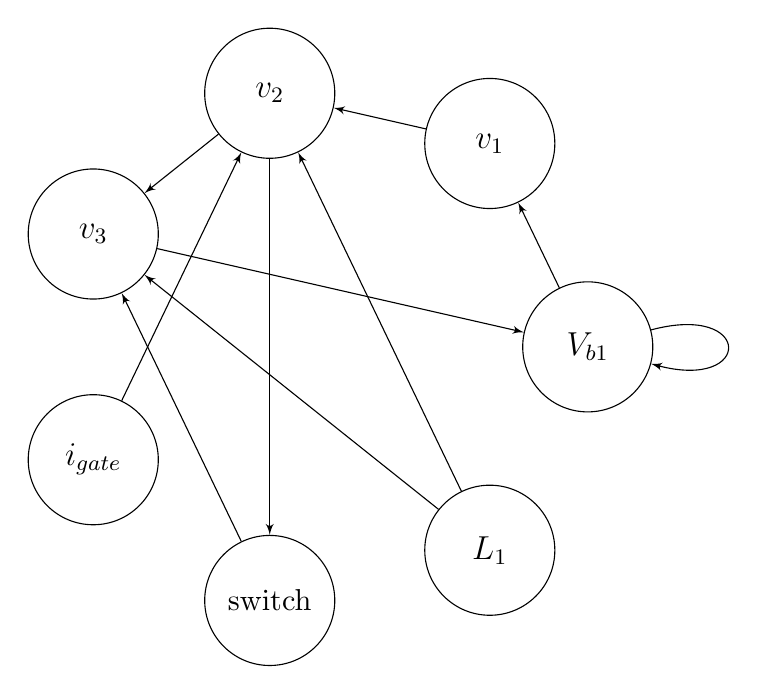
\begin{tikzpicture}[scale=1,auto=center,every node/.style={circle}]
      \tikzset{vertex/.style = {shape=circle,draw,minimum size=4em,fill=white}}
        \tikzset{edge/.style = {->,> = latex'}}
        \def\size{8em}
        % vertices
        \node[vertex] (b1) at  (360/7 * 0:\size) {$V_{b1}$};
        \node[vertex] (n1) at  (360/7 * 1:\size) {$v_1$};
        \node[vertex] (n2) at  (360/7 * 2:\size) {$v_2$};
        \node[vertex] (n3) at  (360/7 * 3:\size) {$v_3$};
        \node[vertex] (r3) at (360/7 * 4:\size) {$i_{gate}$};
        \node[vertex] (s1) at (360/7 * 5:\size) {\small{switch}};
        \node[vertex] (l1) at (360/7 * 6:\size) {$L_1$};
        %edges
        \draw[edge] [loop right] (b1) to (b1);
        \draw[edge] (b1) to (n1);
        \draw[edge] (n1) to (n2);
        \draw[edge] (n2) to (n3);
        \draw[edge] (n2) to (s1);
        \draw[edge] (n3) to (b1);
        \draw[edge] (r3) to (n2);
        \draw[edge] (s1) to (n3);
        \draw[edge] (l1) to (n2);
        \draw[edge]  (l1) to (n3);
    \end{tikzpicture}
    \caption{A dependency graph for some elements and nodes of the nanowire model as presented in
    figure \ref{fig:old_nw}. Each node in the graph represents
    a circuit node value that is calculated or an element parameter.
    Since the compiler is a black box,
    some degree and outdegree $1$ nodes were removed. Note that the time dependence
    of parameters is also removed, i.e. an edge to a variable could represent
    dependence in the same timestep or on the previous timestep of the value.
    This is a heuristic of how simulation parameters
    are dependent on each other, i.e. how stiffness or errors in one graph node couple to other nodes.}
    \label{fig:dependency_graph}
\end{figure}

Using dependency graphs, we can visualize how the model elements
are correlated in figure \ref{fig:dependency_graph}. 
By using directed graphs to represent execution 
order for nodes and element values, we can visualize the dependece
of parameters on each other. A system is said to have a dependency graph $G = (V, E)$
where $V$ represents variables as nodes and $E$ are the dependency edges.
A set of variables $V_1, V_2 \subseteq V$ are said to be decoupled if all nodes
in $V_1$ have node edges pointing to $V_2$ and vice versa. The dependency
graph for a system highlights how projection errors integrate over time.
\todoexplain[]{Explain why cycle, why thermal integrator projections...}
\todoref[]{citation from book Software Testing and Analysis: Process, Principles, and Techniques. Chapter 6}
\todoref[]{dragon book??}
%http://www.cs.toronto.edu/~chechik/courses16/csc410/dataflowReadings.pdf

The current nanowire model also currently lacks a DC part (operational mode) 
of the model.
LTspice DC solver struggles to efficiently represent a nanowire that is
undergoing relaxation oscillations (the solver tends to find that it is
switched) and misrepresents DC solutions for the superconducting state
as the normal state. This implies that for nanowire simulations,
the initial state of everything must be zero since transient analysis relies
on operational point analysis beforehand. Namely, all bias sources,
DC or not, should start at $0$. So a DC bias would be a \cf{PULSE} starting
at 0, ramping to a value and let it rest there for a bit. This is a by-product 
of LTspice not recognizing meta-stable systems. This is tackled by the new 
simulator introduced in section \ref{julia-sim-chapter}.

\subsection{Stability of the original nanowire model}

By varying the relative tolerance and testing different geometries, the value $10^{-6}$
seems to perform the best in terms of stability and accuracy. By testing the LC tank
geometry shown in \ref{fig:tank_circ} using a nanowire and swapping it with a linear 
inductor, we can test several \cf{reltol} values and see if we see the expected 
oscillation behavior. Intuitively, as the relative tolerance value used gets smaller,
the circuit should be ``more correct'' than when allowing for a bigger tolerance.
For the nanowire model, we don't see that behavior. Relative tolerances between $10^{-3}$
and $10^{-7}$
consistently worked in our tests, producing a sinusoidal oscillation. Values
above $10^{-7}$ either switch into the resistive state and lose all the energy immideatly
or oscillate in a decaying fashion. Meanwhile, for the SNSPD readout configuration,
we see consistently better behavior using the malicious circuits method presented in
\ref{malicious_circuits} as we go from $10^{-3}$ to $10^{-6}$ across photon events
and relaxation oscillations.

Even with a \cf{reltol} value of $10^{-6}$, the existing nanowire model is highly unstable
and can be improved through stability analysis.
Using Malicious Circuits, we test multiple operation regimes for
the nanowire and study the stability of every sub-circuit separately. Namely,
we care about the nanowire behavior in 4 different regimes: 
(1) as an inductor and resistor when normal, 
(2) as an inductor when superconducting, (3) the hotspot evolution when a photon is
incident, and (4) relaxation oscillation regime. We test these different regimes 
using one circuit with one nanowire element across \cf{reltol} values of $10^{-3}$
and $10^{-6}$ and compare it to the expected solution.

\subsection{Different Integrator}

The malicious circuits analysis on the old model indicated
that the integrator circuit is the main source of instability. 
We replaced it with a behavioral source that integrates the same hotspot
and observed an improvement in overall behavior.
This model is mathematically identical to the previous one with 2 changes
to the implementation: (1) use a built-in integrator instead of the circuit
integrator (subcircuit c) and (2) replacing $\frac{x+|x|}{2}$ with a conditional
on $x>0$ (or bound $x$ by the \cf{limit}).

The LTspice built-in integrator is better handled
by spice than the integrator's circuit equivalent model.
It involves doing one operation instead of increasing the circuit
matrix size. 
This not only involves creating fewer projections onto the circuit (leading to less errors)
but using the built-in integrator allows LTspice to better keep track of integration
time and shorting to ground. Note that the new integrator using the built-in
\cf{sdt} math command uses a reset condition. This condition is better handles as it
doesn't involve decreasing the timestep in a projective fashion as with circuit
non-linearities. The reset condition is substituting the switch that shorts $v_3$
to ground in figure \ref{fig:old_nw}. When the $v_2=0$ (wire is superconducting),
the integrator resets to the initial condition $0$.

The previous nanowire model also involved the switch toggling between the off and on
state with resistances of $1$m$\Omega$ and $10$G$\Omega$. This switching behavior
introduces a strong non-linearity that can be better handled by the reset method
used by the \cf{sdt} command. In SPICE, a resistance changing value by an order of
$10^6$ instantly is unstable, let alone a magnitude of $10^{15}$. This magnitude
change coupled with using a lower \cf{reltol} leads to a large instability that
should be avoided.

Replacing $\frac{1}{2}\left(x+|x|\right)$ with an IF statement (or limit) allows the circuit matrix compiler to
have an easier time optimizing the simulation. The evaluation of this statement results in $x$ if $x>0$, otherwise
$0$.
While $\frac{1}{2}\left(x+|x|\right)$ preserves continuity,
a carefully crafted IF statement can exhibit the same continuity. This implies that no advantage from a
convergence standpoint is offered, however, the compiler has to perform multiple operations instead of
evaluating one conditional. The limit math command is a built-in way of handling this as well, where the
lower limit is $0$ and the upper limit is the peak hotspot resistance. While the implementation of the limit
command is unknown, its implementation (and accompanying optimization) should intuitively be similar to that
of an IF statement. These two methods also allow for greater readability than the absolute value conditional.

\begin{figure}
    \centering
    \includegraphics[width=0.9\textwidth]{figs/int_improvement_1e-3.png}
    \caption{Comparison of the old and new nanowire model that replaces the
    circuit integrator with the internal LTspice resetting integrator. Solid
    lines represent the output waveform and the crosses are the values evaluated at each
    individual timestep. Photons are incident at $2$ and $32$ns on a wire biased by $15\mu$A.
    The bias is increased to $25\mu$A between $10$ and $30$ns to enter the wire into the
    relaxation oscillation regime.We see that in this example, the new model is more accurate, as well as, requiring fewer discrete timesteps to solve the equation at.}
    \label{fig:int_improvement_1e-3}
\end{figure}

\begin{figure}
    \centering
    \includegraphics[width=0.9\textwidth]{figs/int_improvement_1e-6.png}
    \caption{For the same setup in figure \ref{fig:int_improvement_1e-3}, we see
    that both models seem to perform well on readout when using a \cf{reltol} value
    of $10^{-6}$. However, the hotspot resistance is unstable in the old model peaking
    up to $2$ orders of magnitude above the actual value.}
    \label{fig:int_improvement_1e-6}
\end{figure}

Along with more accurate simulations of the behavior of the nanowire, we also
observe the simulator using fewer time steps overall (fewer crosses in figure 
\ref{fig:int_improvement_1e-3}). This corresponds to faster convergence and also is
an indicator of fewer projections that needed to be done, indicating less
error over the binary state. Needing fewer points to solve a system suggests
linearity. In this case, we can observe that the model can comfortably relax
back into linearity when the pulse magnitude is constant and there is no
switching behavior occurring. The higher density of datapoints in the improved model 
is reserved for the beginning of the state non-linearity transition (hotspot growth region)
as opposed to being employed during the entire evolution in the old model.

Figure \ref{fig:int_improvement_1e-6} compares the performance of the old and new 
nanowire models at a \cf{reltol$=10^{-6}$}. This example is for the same bias as in 
figure \ref{fig:int_improvement_1e-3}, where the current output seems correct.
However, looking at the hotspot resistance by scoping the internal variables of the 
model, we see that the hotspot resistance has huge spikes, up to 2 orders of magnitude
above the correct value. This is a source of instability in the model that can also
be analyzed using Malicious Circuits, even though the hotspot resistance itself is
a combined measurable ($R_{\mathrm{hotspot}} = \frac{v_1 - v_{\mathrm{source}}}{i}$).

\begin{figure}
    \centering
    \includegraphics[width=0.8\textwidth]{figs/not_jumbled_mess.png}
    \caption{A sweep of bias currents on the new nanowire model with a photon detection event.
    $100$ equally spaced bias values between $11\mu$A and $12\mu$A were tested. We observe
    a smooth gradient of the resultant
    hotspot resistance and voltage spike that is much more consistent than the old nanowire
    as shown in figure \ref{fig:sweepbias}. 
    }
    \label{fig:not_jumbled_mess}
\end{figure}

We can see the same sweep performed on the original nanowire in figure \ref{fig:sweepbias}
performed on the model with improved stability in figure \ref{fig:not_jumbled_mess}. We can see
a smooth gradient of responses form as the bias increases (as opposed to random activity seen
in the old model). This is expected, as the device should experience one harsh state non-linearity.
After that transition, the system to should be continuously non-linear in a fashion that can be simulated
by transient simulations accurately. We also can see the hotspot peak resistance increase smoothly
with the bias current in the new model, while witnessing the hotspot decaying faster. This showcases
that our model is directing current to the shunt at a faster rate -- allowing the wire to cool back into the
superconducting state earlier on.

\subsection{1-Element Models}

Collapsing a sub-circuit to one element can provide speed and convergence advantages, especially for
nonlinear elements, at the risk of instability past a certain point. This method can be useful in
applications where the nanowire is used in one configuration repeatedly. For example, in the SNSPI
model generated in section \ref{snspi_dyn_model}, replacing the nanowire element with a behavioral
one-element model that spikes the resistance upon a photon incidence without integrating the entire
hotspot velocity. This can be done by precomputing the effect of the bias in a program like spice-daemon
and reusing that computed value or by loading multidimensional PWL tables into LTspice.

A good resource for one-element models are behavioral sources (b-sources). B-sources can operate
in the voltage (BV source) and current source (BI source) mode with their outputs set by an arbitrary 
maths expression
which can be a function of global parameters such as node values. B-sources can also behave
as behavioral resistors (BR) and power sources (BP), these two modes aren't well documented.
BR sources are useful candidates for modelling hotspots, as they can have a 0 resistance that spikes
to the hotspot peak resistance. The tolerances are more lenient for a BR than a BV source across
a resistor. The nanowire model has a small $10^{-3}\omega$ resistance, which is inconsequential for
most simulations. Care should be taken when using a BR source starting at zero resistance as it
may cause convergence issues if nonlinear effects trigger smaller timesteps near the switching
threshold.

Precomputing switching behavior outside LTspice can be done by modelling any complicated thermal
model in outside software and imported into LTspice via \cf{spice-daemon}. This could involve stripping
nanowires from the hotspot integrator and having voltage spikes output across it as a normal
nanowire would given the bias the resistor is experiencing. Since \cf{spice-daemon} can access
simulation data, the nanowire bias can be deduced either explicitly from the YAML file or by
running an initial DC simulation to determine the nanowire bias.

Multidimensional tables can also be computed for nanowires and imported into LTspice. LTspice doesn't
support 2D tables or interpolation, it only supports 1D piece-wise-linear (PWL) interpolation. This
however can be overloaded using the \cf{mod} function to define a well-convergent 2D interpolation 
space using a 1D mapping. For example, a 2D map on $x, y$ evaluating to $f(x, y)$ can be encoded 
by enumerating each square with the diagonal points $(x, y)$ and $(x+\Delta x, y + \Delta y)$ and 
computing $f$ at the corners of each square. This
enumeration is linear, one general example mapping is $M(x, y) = \frac{1}{k_x}\floor{k_xx}+G\cdot \frac{1}{k_y}\floor{k_yy}$ where
$k_x, k_y$ are related to the resolution ($\Delta x, \Delta y$) and $G$ is related to $\max{x}$
and $k_x$. 
The mapping $M(x, y)$ evaluates to one unique number for each pair $x, y$ on the corners
of the squares. We can now interpolate any function $f$ across that range for any two query points 
$x', y'$ by evaluating
a function $f$ over the points $M(x, y), M(x+\Delta x, y), M(x, y+\Delta y), M(x+\Delta x, y+\Delta y)$.
The weighted sum of these evaluations is a 2D linear interpolation. A different simpler method could be
used (such as rounding) for a 2D table with no interpolation. The basic principle for encoding higher 
order maps into LTspice is to convert
the space to a finite enumerated map, compute the target function over the corners of each square and
encode that using the \cf{table} math command. 

These models require less operations and checks per iteration, allowing for faster compute. 
These models are ideal for large scale simulation, such as simulating thousands of nanowires.
Using
a behavioral source with finitely many operations takes less than 6 operations per iteration and
acts on one node. Even in a sparse setting, arbitrary subcircuits span multiple entries and force
a larger number of operations a second - many resulting from individual \cf{reltol} (and other tolerance)
checks. Using a macro-model to encode the behavior of the nanowire decreases the number of possible
stability issues. However, these macro-models encode a finite number of interactions, and as such, can 
act in a behavior that seems correct (since it is hard coded) when it is not. This motivates being
extra careful with models designed for high performance and large-scale system modeling. Having an
environment controlled check to validate the sensibility of a circuit output is a useful add-on. For
example, having the pre-compute workflow in \cf{spice-daemon} compute the behvioral model and the
post-compute workflow check that when the nanowire switched, the current in the device was above
the critical current, a photon was incident, etc. 
\section{Efficient Simulation} \label{julia-sim-chapter}

\todo[inline]{Julia simulator}

\subsection{Tline Model}

\subsubsection{Equivalent Circuit}

\subsubsection{Kernel}

\subsubsection{GPU}

\subsection{Harmonic Balance} \label{julia-sim-hb}

\subsubsection{TD Assist}

\subsection{Device Symmetries}

\subsection{Coupling Diff. Eq. (or Thermal Model?)}

Maybe sections should be separate. Phonon-Electron transport.

Complex electric coupling

\subsubsection{TDC}

\subsubsection{SNSPI coupling}

\subsection{Precomputation}

\subsection{ML Optimization}

\subsubsection{Symbolic Solver}

\subsubsection{Tapers}

Note on resistive groups? -> Sonnet?

\subsubsection{Differentiable Simulator}

\subsubsection{Inverse design}

\subsubsection{Monte Carlo Simulation}

% \section{Time Domain Reflectometry}

% \subsection{Idea}

% \subsection{Optimal Search Theory}

% \subsection{Simulation}

% \subsection{Experimental Setup}

% \subsection{Results}

% \subsection{Future Ideas}

\newpage

% \bibliographystyle{asmeconf}
\begin{sloppypar}
\printbibliography
\end{sloppypar}

\end{document}
